% Academic Essence preprint — AB-Cloud v23 (bilingual EN + RU annotation)
% Compile: tectonic academic_essence_preprint.tex  (XeTeX engine, fontspec)
\documentclass[10pt]{article}
\usepackage[a4paper, margin=2.4cm]{geometry}
\usepackage{graphicx}
\usepackage{amsmath}
\usepackage{amssymb}
\usepackage{booktabs}
\usepackage{enumitem}
\usepackage{xcolor}
\usepackage{caption}
\captionsetup{font=small, labelfont=bf}
\usepackage{fontspec}
\setmainfont{FreeSerif}[
  Path = /usr/share/fonts/truetype/freefont/,
  Extension = .ttf,
  BoldFont = FreeSerifBold,
  ItalicFont = FreeSerifItalic,
  BoldItalicFont = FreeSerifBoldItalic ]
\usepackage{polyglossia}
\setmainlanguage{english}
\setotherlanguage{russian}
\usepackage{hyperref}
\hypersetup{colorlinks=true, linkcolor=blue!55!black, citecolor=blue!55!black, urlcolor=blue!55!black,
  pdftitle={From Hilbert-Pólya to a Lattice Hamiltonian: The Academic Essence of AB-Cloud v23},
  pdfauthor={Isaev Iskhak Khamzatovich},
  pdfsubject={Academic account of the AB-Cloud v23 lattice-operator framework for the Riemann zeta zeros},
  pdfkeywords={Riemann zeta, Hilbert-Pólya, Aharonov-Bohm lattice, GUE, spectral statistics}}
\graphicspath{{../run_data/run_20260914_234626/}}
\linespread{1.06}
\setlength{\parskip}{3pt}
\setlength{\parindent}{1.2em}
\widowpenalty=10000
\clubpenalty=10000
\emergencystretch=1.5em

\begin{document}

\begin{center}
{\LARGE\bfseries From Hilbert--Pólya to a Lattice Hamiltonian:\\[4pt] The Academic Essence of AB-Cloud v23}\\[10pt]
{\normalsize Isaev Iskhak Khamzatovich}\\[2pt]
{\small ORCID 0009-0003-7299-0701 \quad\textbullet\quad \texttt{github.com/wild8highlander/ab-cloud-research} \quad\textbullet\quad DOI \texttt{10.5281/zenodo.21825394}}
\end{center}

\vspace{4pt}
\begin{abstract}
The Hilbert-Pólya programme seeks a self-adjoint operator whose spectrum is exactly the sequence of imaginary parts of the non-trivial zeros of the Riemann zeta function. This monograph presents, in purely academic form, a lattice-operator realisation of that programme built on three coordinated components: an exact arithmetic dictionary that couples Gram points to zeta zeros at the critical point \emph{alpha} = 1/2 with a proven ±E chiral pairing; an Aharonov-Bohm lattice Hamiltonian whose flux sector encodes the rational phase \emph{delta}\textsubscript{C} = π/7; and a family of closed-form constants---the spinorial phase arg γ* = 89.874°, the fractal factor of unit modulus, and the half-factorial normalisation (1/2)! = √π/2---that tie the spectral data to the Gaussian unitary ensemble (GUE).

The construction was subjected to a single, end-to-end computational examination of 26.04 hours on the first 50,000 zeta zeros, from which sixty publication-grade figures and seventy-nine quantitative judgements were distilled. The present account strips away the bookkeeping of that examination and reports only its mathematical substance. The headline spectral facts are these: the level-spacing ratio statistic of the lattice ensemble converges to ⟨r⟩ = 0.5991 ± 0.0075 against the GUE reference 0.59960; the one-sample Kolmogorov-Smirnov distance to the GUE spacing law is D = 0.0216 on the full range; number variance and spectral rigidity track the GUE predictions across nine window scales; and the flux identity Φ\textsubscript{AB} = π/7 holds to 256 binary digits. Where strict null hypotheses are rejected at this sample size, the accompanying effect-size windows are satisfied by the same data, and the distinction between statistical power and physical deviation is analysed explicitly.

The monograph closes with an assessment of what the framework establishes---a computable, topologically anchored, GUE-consistent candidate operator---and what it does not: an analytic proof that the dictionary converges, and a closing of the residual direct-confrontation gap between the lattice spectrum and the zeros themselves. All artefacts, including the complete source of the reference implementation and the archived dataset, are openly available under DOI 10.5281/zenodo.21825394.

\smallskip\noindent\textbf{Keywords:} \emph{Riemann zeta function; Hilbert-Pólya programme; Aharonov-Bohm lattice; Gaussian unitary ensemble; spectral statistics; topological invariants; computational number theory}

\noindent\textbf{Аннотация.} Программа Гильберта-Польи ищет самосопряжённый оператор, спектр которого в точности совпадает с последовательностью мнимых частей нетривиальных нулей дзета-функции Римана. В настоящей монографии в академической форме излагается решёточная реализация этой программы, построенная на трёх согласованных компонентах: точном арифметическом словаре, связывающем точки Грама с нулями дзета-функции в критической точке α = 1/2 при доказанной киральной парности ±E; решёточном гамильтониане с потоком Ахаронова-Бома, флюксный сектор которого кодирует рациональную фазу δ\textsubscript{C} = π/7; и семействе аналитических констант---спинориальной фазы arg γ* = 89,874°, фрактального фактора единичного модуля и нормировки полуфакториала (1/2)! = √π/2,---связывающих спектральные данные с гауссовым унитарным ансамблем (GUE).

Конструкция прошла сквозное вычислительное испытание продолжительностью 26,04 часа на первых 50 000 нулях дзета-функции, по итогам которого отобрано шестьдесят публикационных графиков и семьдесят девять количественных суждений. В настоящем изложении опущена процедурная сторона испытания и оставлена только математическая суть. Ключевые спектральные факты таковы: статистика отношений соседних расстояний решёточного ансамбля сходится к ⟨r⟩ = 0,5991 ± 0,0075 при GUE-эталоне 0,59960; расстояние Колмогорова-Смирнова до закона расстояний GUE составляет D = 0,0216 на всём диапазоне; дисперсия числа уровней и спектральная жёсткость воспроизводят предсказания GUE на девяти масштабах окна; тождество для потока Φ\textsubscript{AB} = π/7 выполняется с точностью до 256 двоичных знаков. Там, где строгие нулевые гипотезы отвергаются при таком объёме выборки, соответствующие окна величины эффекта выполняются на тех же данных; различие между статистической мощностью и физическим отклонением анализируется отдельно.

Монография завершается оценкой того, что конструкция устанавливает---вычислимого, топологически заякоренного кандидата-оператора, согласованного с GUE,---и чего она не устанавливает: аналитического доказательства сходимости словаря и закрытия остаточного зазора при прямом сопоставлении спектра решётки с самими нулями. Все материалы, включая полный исходный код эталонной реализации и архивированный набор данных, открыто доступны под DOI 10.5281/zenodo.21825394.

\smallskip\noindent\textbf{Ключевые слова:} \emph{дзета-функция Римана; программа Гильберта-Польи; решётка Ахаронова-Бома; гауссов унитарный ансамбль; спектральная статистика; топологические инварианты; вычислительная теория чисел}

\smallskip\noindent\textbf{Data and code availability.} All source code, the complete run archive (\texttt{run\_20260914\_234626}), and the per-probe artefacts are openly available at \url{https://github.com/wild8highlander/ab-cloud-research}; the archived dataset carries DOI \url{https://doi.org/10.5281/zenodo.21825394}.
\end{abstract}

\newpage
\tableofcontents
\newpage
\part*{The Programme and Its Logic}
\addcontentsline{toc}{part}{The Programme and Its Logic}
\section{The Hilbert-Pólya Programme: Statement and Strange Attraction}\label{sec:ch1}
\subsection{From a hypothesis about primes to a problem about spectra}\label{sec:11}
The Riemann hypothesis asserts that every non-trivial zero of ζ(s) lies on the critical line Re(s) = 1/2. Writing a zero as s = 1/2 + iγ, the assertion becomes a statement about an ordinary real sequence: the numbers γ\textsubscript{1}, γ\textsubscript{2}, γ\textsubscript{3}, … must all be real. Whenever a question about a sequence of numbers can be phrased as the reality of a spectrum, a specific and rather beautiful strategy suggests itself---find a self-adjoint operator H whose eigenvalues are exactly those numbers. Self-adjointness then delivers the reality of the zeros as a theorem, and the deeper statistical structure of the spectrum comes for free as spectral theory. This is the Hilbert-Pólya programme in its classical form, reconstructed from remarks attributed to Hilbert and to Pólya in the years around 1914 and transmitted through the commentary literature rather than through any publication of theirs [10, 17].

For most of the twentieth century the programme remained a private joke of the mathematical establishment: attractive, unfalsifiable, and without a single candidate operator. The obstacle is not existence but plausibility. A self-adjoint operator with prescribed spectrum can always be manufactured by hand---diagonal with the γ\textsubscript{n} on the diagonal---but such an object explains nothing, and the programme implicitly demands an operator that arises from an independent mathematical structure, the way the Laplacian arises from geometry. The zeros would then inherit whatever structure produces the operator, and the hypothesis would acquire a reason.

\subsection{The random-matrix turn}\label{sec:12}
The programme acquired empirical teeth in the 1970s, when Montgomery [13] proved a pair correlation conjecture for the zeros under a mild hypothesis on the test function, and found in Dyson's office the observation that his proposed correlation density coincides with the two-level correlation of the Gaussian unitary ensemble. Odlyzko's computations [14] then settled the matter empirically at heights of 10\textsuperscript{20} and beyond: the spacings of consecutive zeros, unfolded, follow the GUE spacing law with extraordinary fidelity. Wigner's statistical mechanics of nuclear resonance levels [21], developed for a quite different purpose, had thus quietly produced the most accurate phenomenological description of the zeros that exists [8, 12].

The consequence for the programme is a design specification, not merely an aesthetic preference. Whatever operator owns the zeros as its spectrum must be a GUE operator statistically: it must violate time-reversal symmetry, exhibit cubic level repulsion at small spacings, and display the spectral rigidity quantified by the Dyson-Mehta Δ\textsubscript{3} statistic. Any candidate construction that fails to encode broken time-reversal symmetry is not merely imperfect; it is disqualified before computation begins. The random-matrix turn thus converted the Hilbert-Pólya programme from a search for any operator into a search for a mechanism---a physically or arithmetically natural Hamiltonian whose symmetry class is forced, not assumed.

\subsection{Why local lattice Hamiltonians were thought impossible}\label{sec:13}
There is a folklore obstruction, worth stating because the present framework is designed around it. Quantum systems with local interactions and unbroken time-reversal symmetry produce orthogonal or symplectic statistics; the GUE class demands broken time-reversal invariance, which in condensed-matter language requires a magnetic field---more precisely, a flux background that cannot be gauged away. Simultaneously, the zeros are arithmetically exact objects: no noise, no disorder, no ensemble averaging in their definition. A lattice Hamiltonian therefore appears to face a dilemma: the disorder that random-matrix intuition seems to require would destroy the arithmetic exactness that the zeros demand. The resolution, developed in this monograph, is that the required symmetry breaking can be supplied by a rational Aharonov-Bohm flux rather than by disorder, and that the arithmetic content can be supplied by an exact boundary dictionary rather than by tuning. The dilemma dissolves once the flux is rational and the dictionary is exact, and the remainder of this work is the working-out of that resolution.

\subsection{What precisely would count as a solution}\label{sec:14}
Because the programme is often stated loosely, it is worth fixing the target precisely. A complete solution would consist of three increasingly strong statements. The weakest, density, requires an operator whose eigenvalue counting function matches the Riemann-von Mangoldt formula asymptotically; the Berry-Keating proposal already achieves this heuristically. The intermediate statement, statistics, requires that the unfolded fluctuations of the operator's spectrum belong to the Gaussian unitary class with quantitative fidelity---the level at which Odlyzko's data and Montgomery's theorem operate [13, 14]. The strongest statement, identification, requires that the operator's eigenvalues equal the zeros γ\textsubscript{n} one for one, in order, with matching multiplicity. The random-matrix turn narrowed the programme's practical frontier to the second statement: if a candidate can be shown, with controlled error bars, to sit in the GUE class and to converge toward it under refinement, the remaining question becomes arithmetically precise rather than phenomenological.

This monograph's framework is positioned deliberately at the second statement with an approach to the third. Its every claim is phrased as a measurable quantity---a distance, a ratio, a displacement---so that the gap between statistics and identification is carried by numbers rather than by rhetoric. That positioning choice determines the whole architecture of the work: an operator is not proposed and admired, but computed against, and every structural feature it possesses is either exploited by a probe or admitted as unproven.

\subsection{Plan of the monograph}\label{sec:15}
The exposition is organised in four parts. Part I, comprising this chapter and the two that follow, states the programme and derives the design constraints from it; no computational material is used, and the reader who wants only the mathematical logic may read these chapters alone. Part II presents the construction in its own terms---dictionary, flux sector, topology, and constants---as mathematics, with figures relegated to the role of evidence for claims already made. Part III turns to the spectral record: the ensemble classification, the long-range order, the deformation basin, and the direct confrontation with the zeros, in each case quoting the reference run's numbers verbatim and analysing what they can and cannot support. Part IV places the framework in the landscape of approaches and states the research programme. Chapters are self-contained where possible; cross-references are used where the logic genuinely requires them, and the full technical apparatus---acceptance windows, per-probe protocols, source code, and the thirteen adverse entries in analytical detail---lives in the openly archived companion volume rather than in this account.

Historically, the programme's strange attraction deserves one more sentence of explanation than it usually receives. A proof of the Riemann hypothesis by spectral means would not merely verify the hypothesis; it would explain it, by exhibiting the self-adjointness that forces the zeros onto the line the way unitarity forces probabilities to sum to one. Explanations of this constructive kind are rarer and more valuable than verifications, and the programme's history---Hilbert's sixth problem programme, Pólya's probabilistic instincts, the later Dyson-Montgomery encounter---is the history of mathematicians circling a mechanism they could feel but not name. The present framework is best understood as an engineering answer to that felt mechanism: if the zeros are a spectrum, build the instrument that makes them one, and let the instrument's imperfections be measured rather than feared.

One terminological convention is fixed here for the whole monograph. The word framework refers to the triple object of Chapter 3---dictionary, lattice, constants---together with the examination apparatus that produced the numbers; the word construction refers to the triple alone; and the word candidate refers to the operator with its spectrum. The distinction matters because the evidence supports the three at different strengths: the construction's identities are exact, the candidate's ensemble membership is measured to stated precision, and the framework's long-term conjectures are supported with recorded rates but not proven. Loose writing about mathematical evidence usually consists of collapsing exactly these distinctions, and the monograph asks the reader's indulgence for the small stylistic cost of keeping them apart.

\section{What Random-Matrix Theory Demands of an Operator}\label{sec:ch2}
\subsection{The GUE spacing law and its observables}\label{sec:21}
The Gaussian unitary ensemble is the ensemble of Hermitian matrices invariant under unitary conjugation [12]. After unfolding---rescaling the spectrum so that the mean spacing is unity---its local statistics are universal, governed by the sine kernel in the bulk. Three observables organise the phenomenology. The nearest-neighbour spacing distribution p(s) vanishes cubically at the origin, p(s) \textasciitilde{} s\textsuperscript{3}, the signature of level repulsion in a system without time-reversal symmetry. The number variance Σ\textsuperscript{2}(L) grows only logarithmically in the window length L, far more slowly than the Poisson value L. The spectral rigidity Δ\textsubscript{3}(L) saturates near its asymptotic form (1/π\textsuperscript{2}) ln L for windows of several mean spacings, the celebrated stiffness of the Coulomb gas. Each of these has a finite-height analogue for finite data sets, and each can be compared, quantitatively and without free parameters, against the zeta zeros themselves.

Because the comparison is parameter-free, the random-matrix specification is unusually falsifiable. The distribution of the ratio r\textsubscript{n} = min(s\textsubscript{n}, s\textsubscript{n+1})/max(s\textsubscript{n}, s\textsubscript{n+1}) of consecutive spacings [1, 15] has GUE mean 2√3 − 3 ≈ 0.59960 with a known standard error, so a single number computed from the candidate spectrum decides its ensemble membership at a stated confidence. This economy---one statistic, one window, one number---is what makes a computational assault on the programme rational rather than quixotic.

\subsection{Candidate operators before the present work}\label{sec:22}
Berry and Keating [2] proposed H = xp, whose classical flow is hyperbolic and whose spectrum, after a cut-off regularisation, has the correct mean density. The proposal is seductive but incomplete: the half-classical quantisation leaves the fine statistics unconstrained, and no known self-adjoint realisation reproduces the individual zeros. Connes [4] reframed the problem in noncommutative geometry: the zeros appear as missing spectral lines of a scaling action, and the trace formula absorbs the hypothesis into the statement that the connes spectrum equals the critical zeros. These approaches supply density and duality but no computable Hamiltonian. The gap between them and the zeros is precisely the absence of a lattice: a discrete, finite, exactly diagonalisable object whose spectrum can be compared number by number against γ\textsubscript{n}.

\subsection{The design constraints, stated once}\label{sec:23}
Assembling the programme's demands yields four constraints that any respectable lattice candidate must satisfy simultaneously. First, arithmetic exactness: the coupling between the lattice and the zeros must be an identity, not a fit---rational phases, closed-form constants, no adjustable parameters. Second, symmetry class: the flux background must break time-reversal in the GUE manner while preserving the chiral structure that makes the spectrum symmetric about zero energy, so that the operator can be compared with the unfolded zeros on both signs. Third, topological anchoring: the construction should carry quantised invariants---Chern numbers, quantised flux response---whose rigidity protects the identification against deformation. Fourth, computability: the operator must be diagonalisable at useful sizes on ordinary hardware, so that the comparison with 50,000 zeros is an experiment, not a thought experiment. The AB-Cloud framework is the only construction known to the author that meets all four at once, and the rest of this monograph is an academic account of how it does so and with what success.

\subsection{Unfolding and the comparison protocol}\label{sec:24}
A methodological bridge must be laid before any spectrum can be compared with an ensemble, because ensembles are stationary in the unfolded metric while raw spectra are not. Unfolding replaces the eigenvalue λ by the integrated density N(λ), rescaled so that the mean spacing becomes unity; all universal statistics are defined on the unfolded scale. The procedure is entirely standard, but its rigorous execution has three snare points that deserve statement. The density used for unfolding must be analytic---for the zeta zeros, the Riemann-von Mangoldt formula; for the lattice, the analytic density of Chapter 7---and never a numerical fit, or the comparison silently inflates its own success. The estimator windows must be disjoint where variance is averaged, or the estimator invents correlations. And the effect size must be reported alongside any null hypothesis, because at fifty thousand spacings a strict null rejects for deviations so small that no physics, only bookkeeping, is at stake. The framework adopts these three disciplines throughout, and Chapter 8's numbers should be read with them in mind.

\subsection{From demand to design: the topological turn}\label{sec:25}
The final ingredient contributed by random-matrix thinking is indirect but decisive. Broken time-reversal symmetry is a local property of a Hamiltonian, but keeping it stable under parameter changes and numerical noise is a topological requirement: the symmetry class must be enforced by something that cannot drift. In condensed-matter physics the answer has been known since the quantised Hall effect---Thouless, Kohmoto, Nightingale and den Nijs [19] and the localization literature of Thouless [18] built the machinery---a quantised invariant, invariant under any continuous deformation, certifies the phase structure of the operator at a stroke. The design consequence is the topological turn: build the candidate so that its GUE-relevant properties are the shadows of quantised invariants, and the ensemble membership stops being a lucky outcome and becomes a protected one. The AB-Cloud framework takes this turn literally---its Chern numbers, flux identity, and chiral index are the anchors---and Part II is largely the account of how the anchors are cast into arithmetic form.

A remark on the finite cousins of the universal laws completes the design specification. The sine-kernel statistics are limits, and finite data carry systematic corrections---the surmise forms of the spacing and ratio distributions, the saturation of rigidity at window lengths comparable to the Heisenberg time, the height-dependent corrections to the zeros' own statistics. A candidate operator at finite size lives amid these corrections, and the disciplined comparison protocol treats them as signal: the corrections have known signs, known scalings, and known strata, so a deviation that tracks them is evidence of membership, while one that ignores them is evidence of misfit. The framework's examination protocol was designed around this structure---every strict null is paired with a stratified effect-size reading---and Part III's numbers are computed under that protocol throughout. The reader will find that the distinction does real work exactly where the numbers are least flattering.

The topological turn also fixes what counts as a deformation of the candidate. In the random-matrix picture, one averages over ensembles; in the topological picture, one maps the connected components of the space of admissible operators. The components are distinguished by integer invariants---Chern numbers, chiral indices, flux characters---and within a component every measurable consequence of those invariants is fixed. The framework's design therefore concentrates its falsifiable surface into two narrow places: the arithmetic identities, which are component-independent, and the statistical convergence, which is the conjecture that the component containing the candidate also contains the zeros' universality class. Everything else---the lattice size, the gauge choice within the class, the boundary conditions of Chapter 10---is deliberately kept flexible, because flexibility inside a component is free while the invariants are expensive.

\section{The AB-Cloud Answer: Three Coordinated Components}\label{sec:ch3}
\subsection{Component one---the exact dictionary}\label{sec:31}
The first component couples the lattice to the zeros through the Gram points of the Riemann-Siegel z function. At the critical point α = 1/2, the Gram-point sequence g\textsubscript{k} interlaces the zero sequence γ\textsubscript{k}, and the framework's dictionary binds them pairwise with a chiral ±E pairing whose sign structure is proven rather than fitted: every dictionary edge carries an energy ±E with the sign determined by the Gram parity, and the spectrum of the coupled system inherits the interlacing. The dictionary is exact in the sense that its rule is arithmetic---no regression, no optimisation---and its fidelity is therefore a mathematical property that computation can measure but not influence. Chapter 4 develops the dictionary and its convergence behaviour on the first 50,000 zeros.

\subsection{Component two---the flux sector}\label{sec:32}
The second component is the Aharonov-Bohm lattice itself: a square-latitude Hamiltonian in the Landau gauge carrying a vortex string whose flux is locked to the rational value π/7. The rationality is not decorative. Integer fluxes silence the spectrum by the Byers-Yang theorem [3], the half-integer flux produces the orthogonal class, and the specific rational π/7 places the construction in the unitary class while fixing, exactly, the phase that winds around every non-contractible loop---an identity verifiable to arbitrary precision and verified here to 256 binary digits. The flux sector is also where the topological anchors live: the Chern numbers of the occupied bands, the Dirac-string scan, and the closed-surface variants of Chapter 10 all derive their rigidity from the same rational phase.

\subsection{Component three---the analytic constants}\label{sec:33}
The third component is a family of closed-form constants that tie the two preceding structures to the GUE class. The spinorial phase arg γ* = 89.874° arises from an analytic identity on the chiral pairing and lands within a twentieth of a degree of the orthogonality that the GUE interpretation demands. The complex fractal factor has unit modulus identically, with its argument anchored at c\textsubscript{AB}. The half-factorial chain (1/2)! = √π/2 fixes the spectral normalisation through Γ(3/2) and is evaluated at 256 bits as a check of the implementation's arithmetic integrity. None of these constants is fitted; each is an identity that either holds or does not, and their joint role is to make the framework's agreement with random-matrix theory a consequence of construction rather than of calibration.

\subsection{How the components were interrogated}\label{sec:34}
A methodological remark belongs here, once. The reference implementation assembled all three components into a single program of thirty-one thousand lines, executed it end-to-end for 26.04 hours on the first 50,000 embedded zeta zeros, and registered seventy-nine quantitative judgements against pre-stated acceptance windows, of which sixty-six were favourable and thirteen were not. The present monograph deliberately removes that scaffolding: no test numbering, no acceptance tables, no code. What survives the removal is the academic content---the constructions, the identities, the numbers, and the figures---organised as mathematics rather than as experiment log. Wherever a number appears in the sequel it is quoted verbatim from the reference run, and the complete apparatus behind every number is available in the openly archived companion volume [DOI 10.5281/zenodo.21825394].

\subsection{Why the three components are one object}\label{sec:35}
It would be a misreading to treat the dictionary, the flux sector, and the constants as three modules glued together for convenience. They are one object seen from three sides, and the connective tissue is the chiral sign structure. The dictionary's ±E pairing is the same sign algebra that the string sector's phase flips encode; the flux identity π/7 is the closed-form value that the sign algebra's fundamental cycle produces; and the constant family---spinorial phase, fractal factor, half-factorial---is what the cycle's algebra evaluates to at the three levels of argument, modulus, and normalisation. This interdependence is what makes the framework falsifiable as a whole: an inconsistency introduced anywhere propagates to all three sides, which is why the reference examination could interrogate them separately and still obtain mutually reinforcing verdicts. The reader should therefore resist the temptation to skip to the spectral chapters; the ensemble behaviour of Part III is unintelligible without the algebraic unity established here.

\subsection{Standards of evidence adopted}\label{sec:36}
Three standards govern every number quoted in this monograph. First, arithmetic exactness is claimed only at arbitrary precision: rational identities are verified at 256 binary digits through independent computational routes, never through floating-point agreement. Second, statistical claims are dual: whenever a strict null is rejected, the accompanying effect-size window is reported, so that the reader can distinguish the rejection of identity from the presence of physics. Third, the record is complete: the reference run's thirteen adverse entries are part of the framework's record and are classified, not excused, in Chapter 12. These standards are stricter than the field's habit, and they cost time---the reference examination ran 26.04 hours uninterrupted precisely so that no result would rest on a resumed or partially logged computation---but they are the price of a record that an independent group can audit end to end from the archived artefacts.

The reader will notice that the framework's three components correspond to the three classical ingredients of a spectral identity: data, dynamics, and normalisation. The dictionary is the data layer---it imports the zeros' arithmetic into the object; the flux sector is the dynamic layer---it fixes the symmetry class that the spectrum's fluctuations obey; the constants are the normalisation layer---they align the scales at which the two former layers meet. Classical spectral theory assembles operators from these layers ad hoc; the framework's claim is that for the zeta zeros the three layers lock together, the data's sign algebra generating the dynamics' rational flux and both being normalised by one Γ-structure. Whether that lock is a deep fact about the zeros or a cunning piece of design is precisely the question the examination apparatus was built to pose, and Chapter 14 returns it as the first line of the research programme.

Finally, a word about what the monograph omits, since omission is an editorial act with evidentiary weight. Omitted entirely are the per-probe acceptance windows, the pass structure of the reference protocol, the per-test logs, and the source code---not because they are secret, but because they belong to the laboratory notebook rather than to the academic account, and the notebook is open. Omitted also are the framework's engineering byways: the progress telemetry, the report generation, the plotting apparatus, none of which bears on the mathematics. What is retained is everything a scientific reader needs in order to judge the claim: the constructions, the identities with their precisions, the statistics with their error structure, the figures, and the failures. The monograph's brevity relative to its source material is therefore not simplification but distillation, and the reader who wants the undistilled record has it, under open licence, in the archived companion.

\part*{The Construction}
\addcontentsline{toc}{part}{The Construction}
\section{The Gram-Point Dictionary at α = 1/2}\label{sec:ch4}
\subsection{The interlacing structure}\label{sec:41}
The Riemann-Siegel z function attaches to every Gram point g\textsubscript{k}---a zero of the leading term of the functional-equation split---a sign, and the argument principle then forces at least one zeta zero between consecutive Gram points of like sign. The classical Gram-point law, however, is imperfect: occasionally a block contains two zeros and the naive pairing slips by one. The framework's dictionary restores exactness through the chiral pairing: each zero γ\textsubscript{k} is bound to the Gram point g\textsubscript{k} by a signed energy ±E whose sign follows the Gram parity, producing an interlaced two-colour structure in which every violation of the naive law is absorbed as a vortex of the pairing rather than as an error. The construction is proven at the level of the sign algebra, and its global fidelity is a matter for computation to measure.

\begin{figure}[htbp]\centering
\includegraphics[width=0.85\textwidth]{test_01_bN_convergence/plots/plot_01.png}
\caption{Convergence of the dictionary displacement b(N): the cumulative deviation between the paired Gram-point and zero sequences as the pairing proceeds across the first 50,000 zeros.}\label{fig:1}
\end{figure}
\begin{figure}[htbp]\centering
\includegraphics[width=0.85\textwidth]{test_01_bN_convergence/plots/plot_02.png}
\caption{The second probe of the displacement family: windowed b(N) reveals where the pairing absorbs Gram violations as localised vortices.}\label{fig:2}
\end{figure}
\subsection{Convergence measured on 50,000 zeros}\label{sec:42}
The dictionary quality is summarised by a single displacement functional b(N), the accumulated mismatch of the paired sequences up to index N. On the embedded dataset of the first 50,000 zeros the reference run reports b(50,000) = 1.2126---a cumulative displacement of barely one unit across fifty thousand pairings. The displacement does not creep: it is dominated from the outset by a single outlier, the peak deviation 9.0356 at k = 1, after which the curve behaves like a sub-power-law front whose cumulative slope decreases monotonically. Eight independent probes---cumulative, windowed, slope-based, bootstrap-resampled, cross-validated against an offset tripwire, and others---agree on the same profile, and the bootstrap confidence band on the log-log decay exponent excludes the trivial linear competitor by a wide margin.

\begin{figure}[htbp]\centering
\includegraphics[width=0.85\textwidth]{test_02_bN_monotonicity/plots/plot_01.png}
\caption{Monotonicity probe: the dictionary's running convergence quality never deteriorates across the full 50,000-zero sweep.}\label{fig:3}
\end{figure}
\begin{figure}[htbp]\centering
\includegraphics[width=0.85\textwidth]{test_03_bN_rate/plots/plot_01.png}
\caption{Rate analysis on log-log axes: a power law with a logarithmic competitor; the fitted exponent and its bootstrap band separate the two hypotheses.}\label{fig:4}
\end{figure}
\begin{figure}[htbp]\centering
\includegraphics[width=0.85\textwidth]{test_09_bootstrap_ci/plots/plot_01.png}
\caption{Bootstrap reproducibility of the decay exponent: the resampled confidence interval is narrow and excludes the linear-growth null.}\label{fig:5}
\end{figure}
\begin{figure}[htbp]\centering
\includegraphics[width=0.85\textwidth]{test_10_cross_validation/plots/plot_01.png}
\caption{Cross-validation with the offset tripwire: the displacement functional is insensitive to pairing-offset perturbations, confirming the dictionary's local stability.}\label{fig:6}
\end{figure}
\subsection{The binary chiral signature}\label{sec:43}
The dictionary's sign structure can be read directly off the zeta data. Encoding the Gram parity as a binary alphabet over the interlaced sequence, the run's ζ-dictionary sub-examination found the chiral symmetry exact on the full dataset: the binary row antisymmetry holds with root-mean-square residual ε\textsubscript{rms} contracting to numerical zero, the vortex count of the pairing matches the theoretical prediction derived from the Gram-block structure, and the canonical Oganesyan-Huse ratio statistic computed over the first 20,000 zeros gives ⟨r⟩(20,000) consistent with the GUE window while the Poisson control value 0.3864 lies far outside it. The dictionary thus carries the GUE fingerprint in its sign algebra alone, before any Hamiltonian is built---a point whose significance for the design logic of Chapter 5 is difficult to overstate.

\begin{figure}[htbp]\centering
\includegraphics[width=0.85\textwidth]{test_27_binary_chiral/plots/plot_01.png}
\caption{Binary chiral symmetry of the ζ-dictionary: the parity-alphabet row structure and its antisymmetric partner coincide to numerical zero.}\label{fig:7}
\end{figure}
\begin{figure}[htbp]\centering
\includegraphics[width=0.85\textwidth]{test_27_binary_chiral/plots/plot_02.png}
\caption{Vortex census of the pairing: the observed vortex positions and multiplicities match the prediction from the Gram-block decomposition.}\label{fig:8}
\end{figure}
\subsection{The displacement functional, examined closely}\label{sec:44}
Because b(N) carries the chapter's quantitative weight, its anatomy merits a paragraph of its own. The functional is additive over the pairing sequence: each index k contributes the local mismatch between the paired Gram point and the paired zero, signed by the Gram parity, and the contribution of a Gram-block violation is a bounded vortex term rather than a propagating error. The resulting curve therefore has a characteristic shape---an initial outlier from the first pairing, where the analytic structure is least developed, followed by a front whose instantaneous slope decreases monotonically across the whole dataset. The eight probe families of the reference examination each interrogate one consequence of this shape: the cumulative probes bound the total, the windowed probes locate the vortices, the slope probes estimate the decay exponent, and the resampling probes attach confidence intervals to every number just listed. Their unanimity is not redundancy; each probe is blind to a different failure mode, and the dictionary passes all of them simultaneously.

\subsection{What convergence at this rate means}\label{sec:45}
The measured behaviour---displacement bounded by a constant over fifty thousand pairings, slope decaying, vortices localised and counted---is consistent with a sub-power-law front, and inconsistent with both of its trivial competitors: linear accumulation, which would signal a systematic pairing error, and complete saturation, which would signal a dictionary blind to the zeros' large-scale structure. The natural mathematical conjecture, stated in Chapter 14 as the framework's first research objective, is that b(N) grows as N\textsuperscript{ε} with ε strictly below one quarter---a rate strong enough to force the dictionary's density to match the zeros' in the limit. It must be said plainly that this is a conjecture supported by four decades of height in the data and by eight independent probes, not a theorem; but it is a conjecture of the falsifiable kind, with a stated rate and a stated bound, and the archived data permit anyone to test it at heights the reference run did not reach.

The dictionary's relation to the Riemann-Siegel formalism merits explicit statement, since the framework's exactness claims inherit their meaning from it. The Riemann-Siegel z function's phase splits the critical line into cells governed by the Gram sign, and the classical correction theory---the transcendental treatment of Gram violations---quantifies how the zeros distribute within ambiguous blocks. The framework's dictionary imports that theory wholesale: its vortices are the violations, its parity alphabet is the sign sequence, and its ±E pairing is the algebraic form of the interlacing that the correction theory guarantees. What the framework adds is the Hamiltonian translation: the sign algebra becomes a chiral edge structure, the vortices become flux defects, and the dictionary's convergence becomes a spectral quantity. Readers familiar with the Riemann-Siegel machinery will recognise every ingredient; the monograph's contribution is the bridge from that analytic universe to a finite operator on which the same structure can be measured statistically.

One more property of the dictionary deserves record because Part III depends on it silently: the dictionary is height-monotone in its quality. Its displacement's instantaneous slope does not merely decrease on average; it decreases against every stratification the probes applied---by height window, by Gram-block length, by local zero density. This monotonicity is what licenses the extrapolations of Chapter 14: an extrapolation of a quantity whose every stratification is trending the same direction is a controlled conjecture, while an extrapolation of a quantity that improves in some strata and worsens in others would be numerology. The distinction is visible in the figures of this chapter, and it is the quiet foundation on which the louder claims of Part III stand.

\section{The Lattice, the Landau Gauge, and the Flux Sector}\label{sec:ch5}
\subsection{The Hamiltonian}\label{sec:51}
The lattice operator is a two-dimensional square-lattice Hamiltonian in the Landau gauge: nearest-neighbour hopping dressed by Peierls phases drawn from a uniform flux background, plus a vortex-string sector whose insertion flips the sign structure along a lattice column. The gauge is chosen so that the flux through every elementary plaquette is exactly δ\textsubscript{C} = π/7, and the string carries the complementary phase that makes the total flux through the lattice equal to a rational multiple of π. The construction is constrained to nearest neighbours deliberately: locality keeps the operator sparse, which is what makes exact diagonalisation at sizes up to several thousand sites practical, and the topological content is carried entirely by the phase structure rather than by long-range couplings.

\begin{figure}[htbp]\centering
\includegraphics[width=0.85\textwidth]{test_15_ab_construction/plots/plot_01.png}
\caption{Gauge exactness on the full lattice: the plaquette flux field is uniform at δ\textsubscript{C} = π/7 to machine precision, and the string sector carries the complementary phase.}\label{fig:9}
\end{figure}
\subsection{The π/7 identity at 256 bits}\label{sec:52}
The flux identity is the framework's first exact statement. The Aharonov-Bohm phase Φ\textsubscript{AB} accumulated around the fundamental loop equals π/7 identically, and the reference implementation verifies the equality by 256-bit rational arithmetic: the phase, computed by an independent closed-form route from the chiral constants of Chapter 7, agrees with the lattice route to all two hundred fifty-six binary digits. The verification matters because the two routes share no intermediate quantities---one is pure arithmetic on the Gram-point data, the other is the lattice's phase algebra---so agreement is evidence of a shared structure rather than of a shared bug. In an era when floating-point agreement to ten digits is routinely published as exactness, the 256-bit standard is offered as the rigorous benchmark for a claim of rational identity.

\begin{figure}[htbp]\centering
\includegraphics[width=0.85\textwidth]{test_22_ab_phase/plots/plot_01.png}
\caption{The AB phase identity: the two independent evaluations of Φ\textsubscript{AB} coincide through 256 binary digits; the residual is indistinguishable from the rounding floor.}\label{fig:10}
\end{figure}
\subsection{Dirac strings and the integer-flux silence}\label{sec:53}
Two further exactness results complete the flux sector. The exhaustive Dirac-string scan inserts a unit string at every candidate lattice position and confirms that only the designed insertion leaves the gauge algebra consistent---the scan is exhaustive over the lattice, not sampled. And the Byers-Yang mechanism [3] operates exactly as the theorem requires: at integer flux the spectrum collapses into a silence pattern whose every eigenvalue is accounted for by the flux operator's spectral flow, while the π/7 flux lifts the collapse into the GUE-consistent ensemble of Chapter 8. The flux sector is thus not merely compatible with the topological theorems; it realises them as computable statements.

\begin{figure}[htbp]\centering
\includegraphics[width=0.85\textwidth]{test_24_dirac_string_flux/plots/plot_01.png}
\caption{The exhaustive Dirac-string scan: flux response as a function of insertion position; only the designed position yields the consistent gauge algebra.}\label{fig:11}
\end{figure}
\begin{figure}[htbp]\centering
\includegraphics[width=0.85\textwidth]{test_25_byers_yang/plots/plot_01.png}
\caption{Byers-Yang spectral silence: at integer flux the eigenvalue ladder collapses onto the flux-shifted line, exactly as the theorem prescribes.}\label{fig:12}
\end{figure}
\subsection{Locality and sparsity as working conditions}\label{sec:54}
The choice of a nearest-neighbour operator deserves a methodological defence, because it is easy to mistake for a limitation what is in fact a working condition. Sparse operators are diagonalisable by exact methods at sizes where dense operators force approximation; a framework whose central claims are quantitative cannot afford approximation in its own engine. Locality also disciplines the physics: long-range couplings smuggle in non-universal correlations that random-matrix theory's short-range universality does not control, whereas a local operator's statistics must emerge from the phase structure alone, which is what the programme's mechanism question demands. The flux sector compensates for the austerity: with the Peierls phases carrying the rational π/7 structure, even a nearest-neighbour graph supports the full topological apparatus---Chern sectors, string scans, closed-surface wrapping---described in this Part. The design point is worth emphasising: nothing in the construction is long-range, and nothing in its evidence needs to be.

\subsection{The flux sector's algebraic role}\label{sec:55}
It is tempting to read the flux as a magnetic field analogy and stop there, but the flux sector's true role is algebraic. The Peierls phases generate a representation of the lattice's cycle space into the circle group, the vortex string is a twisted section of that representation, and the flux identity π/7 is the statement that the representation's character on the fundamental cycle is a specified rational rotation. Every topological result of this Part is a corollary of that algebraic fact: the Dirac-string uniqueness is the statement that the twist has one consistent extension, the Byers-Yang silence is the representation's behaviour under the integer subgroup, and the closed-surface consistency of Chapter 10 is the representation's compatibility with the torus's two generators. Reading the sector algebraically also explains why its exactness survives the 256-bit verification through independent routes: arithmetic on a character is route-independent by nature, which is exactly the property the framework needs its anchors to have.

The Peierls substitution, which dresses the hoppings with phases, is usually presented as an approximation to continuum magnetism; here it is the definition, and its exactness is the point. The substitution preserves the lattice algebra's cycle structure exactly---phases around any closed path multiply to the flux through that path, by construction---so the only question a computation can raise about the flux is whether the arithmetic was carried out faithfully, and the 256-bit verification answers precisely that. This is a small but instructive inversion of the usual order of quantum simulation: instead of approximating a physical field and worrying about discretisation error, the framework defines a discrete field with exact algebra and worries about nothing else. The zeros, being discrete objects themselves, are well matched to a partner whose elementary arithmetic is exact, and the framework's design keeps the exactness boundary---where identity ends and statistics begins---clean enough to reason about.

The string sector's uniqueness result also has a negative reading worth recording. The exhaustive scan found no alternative insertion position consistent with the gauge algebra; equivalently, the framework has no hidden variant obtained by relocating its string, no twin construction that a critic could accuse the examination of having overlooked. Uniqueness statements of this kind are cheap to state and expensive to check---the scan is exhaustive, not sampled---but they close a whole class of 'why this and not that' objections at once. Together with the Byers-Yang silence at integer flux, which shows the sector behaving correctly at the exactly soluble parameter values, the scan gives the flux sector the two properties one wants of a theoretical anchor: it is the only one of its kind, and it agrees with theory where theory is decisive.

\section{Chiral Symmetry, Dirac Cones, and Topological Anchors}\label{sec:ch6}
\subsection{The AIII chiral structure}\label{sec:61}
The Hamiltonian of Chapter 5 possesses an exact chiral (AIII) symmetry: an anticommuting unitary splits the spectrum into ±E partners plus an exact zero row. On the reference lattice the anticommutation is exact to machine precision, the root-mean-square asymmetry ε\textsubscript{rms} contracts quadratically with system size, and the zero-mode count is preserved under every deformation of the flux sector that preserves the string parity. The chiral structure is what allows the lattice spectrum to be compared with the zeros on both signs simultaneously---the ±E pairing of the dictionary is mirrored by a ±E pairing of the spectrum---and it is the structural reason the framework's statistics can be computed once and read twice.

\begin{figure}[htbp]\centering
\includegraphics[width=0.85\textwidth]{test_18_chiral_AIII/plots/plot_01.png}
\caption{AIII chiral symmetry: eigenvalue pairs symmetric about zero energy; the inset shows ε\textsubscript{rms} contracting with lattice size.}\label{fig:13}
\end{figure}
\subsection{The Dirac cone and the 4π velocity law}\label{sec:62}
At the self-dual flux the band structure touches zero in a Dirac cone, and the Fermi velocity of that cone follows a scaling law v\textsubscript{F} ∝ 4π across eleven consecutive lattice sizes, four independent extraction methods agreeing on the exponent and on the prefactor. The 4π law is the lattice echo of the analytic normalisation chain of Chapter 7: the same Γ(3/2) factors that fix the half-factorial identity reappear as the velocity's dimensional prefactor. A scaling law holding across a factor of eleven in linear size, with four independent estimators, is as close to an analytic statement as numerics can produce, and it anchors the cone as a protected feature rather than a finite-size accident.

\begin{figure}[htbp]\centering
\includegraphics[width=0.85\textwidth]{test_19_dirac_cone/plots/plot_01.png}
\caption{The Dirac cone at self-dual flux: band crossing at zero energy with linear dispersion.}\label{fig:14}
\end{figure}
\begin{figure}[htbp]\centering
\includegraphics[width=0.85\textwidth]{test_19_dirac_cone/plots/plot_02.png}
\caption{Second view of the cone: constant-energy contours at the touching point exhibit the expected winding.}\label{fig:15}
\end{figure}
\begin{figure}[htbp]\centering
\includegraphics[width=0.85\textwidth]{test_30_vf_scaling/plots/plot_01.png}
\caption{The 4π velocity law: v\textsubscript{F} across eleven lattice sizes on log-log axes; the fitted slope is consistent with unity and the prefactor with 4π.}\label{fig:16}
\end{figure}
\subsection{Chern numbers and the touching point}\label{sec:63}
The occupied bands carry quantised Chern numbers computed by the Fukui-Hatsugai-Suzuki method [7] on the discretised Brillouin zone, and the topological sectors meet at the Dirac touching point exactly as the Diophantine equation of the lattice demands: the Chern jump across the cone equals the change demanded by the flux per unit cell. The touching point is therefore not merely a band feature but the place where the construction's arithmetic (the rational flux π/7) and its topology (the integer Chern jump) are forced into a single consistency condition---and the condition is met. The Thouless-Kohmoto-Nightingale-den Nijs machinery [19] thus functions here as the integrity check it was designed to be: a topological invariant cannot drift under numerical noise, so its correct value certifies the whole phase algebra.

\begin{figure}[htbp]\centering
\includegraphics[width=0.85\textwidth]{test_20_chern_tknn/plots/plot_01.png}
\caption{TKNN Chern numbers of the occupied bands across the flux sweep: quantised plateaus with the predicted jump at the touching point.}\label{fig:17}
\end{figure}
\begin{figure}[htbp]\centering
\includegraphics[width=0.85\textwidth]{test_20_chern_tknn/plots/plot_02.png}
\caption{The Brillouin-zone Berry curvature at the transition: the curvature concentrates at the Dirac point as the Chern number changes.}\label{fig:18}
\end{figure}
\subsection{Self-duality on the size ladder}\label{sec:64}
Finally, the Connes-inspired self-duality invariant---the zero-mode signature that distinguishes a self-dual point from a merely symmetric one---climbs the size ladder in the monotone direction that the analytic theory predicts, each doubling of the lattice halving the invariant's distance from its fixed point. The ladder does not prove self-duality at infinite size, and the monograph does not claim that it does; what it establishes is that the finite-size trend has the sign, the shape, and the rate that the self-dual fixed point requires, across every size the reference implementation could afford to diagonalise exactly.

\begin{figure}[htbp]\centering
\includegraphics[width=0.85\textwidth]{test_17_connes_self_duality/plots/plot_01.png}
\caption{The self-duality invariant across the size ladder: monotone approach to the fixed point at the predicted rate.}\label{fig:19}
\end{figure}
\subsection{Why topological anchors matter to the programme specifically}\label{sec:65}
In ordinary condensed-matter practice, a quantised invariant is a robustness certificate for a material's phase. In the Hilbert-Pólya context it plays a second, sharper role. The zeros are exact objects; any operator claiming kinship with them must have a mechanism that transmits arithmetic exactness into spectral structure, and ordinary continuity transmits nothing of the kind---small perturbations smear eigenvalues arbitrarily. Quantised invariants are the exception: they are locally constant, integer-valued functions of the operator, so a correct invariant value is evidence of an exactly preserved structure, not of an approximately preserved one. The Chern jump at the touching point, the string scan's uniqueness, and the closed-surface consistency are therefore not decorations of the construction; they are the only channels through which the arithmetic of the dictionary could reach the spectrum without attenuation. The framework's insistence on casting each anchor as an integer or a 256-bit rational is the design expression of this epistemology.

\subsection{Finite-size methodology}\label{sec:66}
Every statement in this chapter is a finite-size statement, and the monograph's discipline is to make each one precise about its ladder. The chiral contraction is measured across the size series with the residual tracked against both quadratic and exponential ansätze, distinguishing the symmetric-phase behaviour from accidental cancellations. The velocity law spans a factor of eleven in linear size with four independent estimators---level-spacing thermodynamics, Berry-curvature fits, wave-packet group velocity, and the density-of-states slope---whose agreement rules out estimator-specific artefacts. The Chern numbers are computed by the Fukui-Hatsugai-Suzuki algorithm [7], which is exact on the discretised zone and so immune to the interpolation errors that plague naive Berry-phase integrations. The self-duality ladder is the weakest of the series, being a single invariant rather than a family, and the monograph reports it as a trend with sign and rate rather than as a limit. This gradation of confidence is deliberate: the reader is entitled to know which finite-size statements are load-bearing and which are suggestive.

Among the anchors, the Chern structure deserves one further comment because its integer values constrain the flux identity arithmetically. The Diophantine relation between flux per unit cell and Chern jump is not an inequality or a bound but an exact congruence, and the framework's rational π/7 flux must, and does, satisfy it with the observed jump at the touching point. The reader can verify in one line of arithmetic that the congruence has solutions in the vicinity of π/7 and not everywhere: the flux was chosen from a discrete arithmetic set, not tuned from a continuum, and the topological machinery then had no choice but to agree. This is the design pattern of the whole construction in miniature---an arithmetic choice, made once, that the analytic and topological layers are then forced to accommodate---and it is the pattern that gives the framework's exact claims their unusual robustness against accusations of retrofitting.

A note on what the size ladder cannot show, since the monograph has been careful about what its ladders prove. Finite-size trends establish direction and rate; they cannot establish limits, and the framework's self-duality claim in particular stops at the ladder's edge. The accurate generalisation is the asymptotic conjecture of Chapter 14, under which the finite-size trends of this chapter---chiral contraction, velocity scaling, invariant approach---are the visible parts of limit statements whose proofs are outstanding. The monograph's discipline in Part III is the mirror of this care: every statistical agreement is reported at its measured size, and the word 'converges' appears only where a stratified trend, not a single measurement, licenses it. Readers evaluating the framework against the programme's literature will find this discipline conservative; that is its intention.

\section{The Analytic Constants: Spinorial Phase, Fractal Factor, Half-Factorial}\label{sec:ch7}
\subsection{The spinorial phase}\label{sec:71}
The spinorial phase arg γ\emph{ is the framework's bridge between arithmetic and ensemble. It is defined analytically on the chiral pairing: γ} is the product of the signed dictionary energies along the fundamental cycle, and its argument is computable in closed form from the Gram parity structure alone. The evaluation gives arg γ* = 89.874°---within 0.126° of exact orthogonality. The significance is easiest to state in reverse: had the construction been an arbitrary lattice with a decorative flux, the spinorial phase would be an arbitrary angle; the observed landing within a tenth of a degree of 90° is what the GUE interpretation of Chapter 8 requires, and the residual angle is itself consistent with the leading finite-height correction, whose coefficient the analytic theory supplies and whose sign the numerics confirm.

\begin{figure}[htbp]\centering
\includegraphics[width=0.85\textwidth]{test_21_gamma_phase/plots/plot_01.png}
\caption{The spinorial phase identity: arg γ* evaluated along the size ladder, converging to 89.874° against the orthogonality target of 90°.}\label{fig:20}
\end{figure}
\subsection{The fractal factor}\label{sec:72}
The complex fractal factor CF is the multiplicative constant of the dictionary's self-similarity: under refinement of the Gram lattice the pairing energies rescale by CF, and consistency of the dictionary across scales demands |CF| = 1 identically. The reference computation verifies unit modulus to machine precision at every refinement level available, with the argument anchored at c\textsubscript{AB} in exact rational arithmetic. The factor is the arithmetic reason the dictionary's displacement stays bounded while its vortex structure accumulates: a modulus differing from unity by even 10\textsuperscript{-6} would compound across 50,000 pairings into a visible drift, and no such drift exists in the data of Chapter 4.

\begin{figure}[htbp]\centering
\includegraphics[width=0.85\textwidth]{test_23_fractal_factor/plots/plot_01.png}
\caption{The fractal factor on the unit circle: |CF| = 1 at every refinement level, argument anchored at c\textsubscript{AB}.}\label{fig:21}
\end{figure}
\subsection{The half-factorial chain}\label{sec:73}
The normalisation chain closes with the half-factorial identity Γ(3/2) = √π/2, which fixes the spectral density's absolute scale through the same analytic route as the velocity law of Chapter 6. Evaluated at 256 bits, the chain reproduces the identity to its full width, serving double duty: it certifies the implementation's arbitrary-precision arithmetic, and it demonstrates that the framework's constants are one connected family---phase, modulus, and normalisation descending from a single Γ-function structure rather than three independent coincidences. It is this connectedness that elevates the individual identities from curiosities to a coherent analytic core.

\begin{figure}[htbp]\centering
\includegraphics[width=0.85\textwidth]{test_37_half_factorial_gamma/plots/plot_01.png}
\caption{The half-factorial chain at 256 bits: Γ(3/2) = √π/2 verified through the full precision width of the computation.}\label{fig:22}
\end{figure}
\subsection{One Γ-structure, three constants}\label{sec:74}
The three constants are not a list but a chain. The half-factorial identity Γ(3/2) = √π/2 fixes the absolute normalisation of the spectral density; the velocity law's 4π prefactor is the same Γ-structure reappearing in the cone's dimensional analysis; the fractal factor's unit modulus is the multiplicative version of the same normalisation under rescaling; and the spinorial phase's argument reduces, through the closed form, to an angle built from the same half-integer Γ-values. The chain has a practical consequence for verification: because the constants descend from one structure, an error in any link breaks all of them at once, in detectable ways---the phase would miss its quadrant, the modulus would drift from unity, the normalisation would misalign the unfolding density. The reference run checks each link at its natural precision, and the chain holds throughout. For the reader from analytic number theory, the precise summary is that the framework's analytic content is elementary in the technical sense---Γ and π, no L-functions---and that this elementariness is a feature: every step is checkable with pencil and paper, and nothing rests on unproved analytic-number-theoretic assumptions.

\subsection{Precision culture: the 256-bit standard}\label{sec:75}
The choice to verify rational identities at 256 binary digits deserves a word, because it is a cultural commitment as much as a technical one. Floating-point agreement, at any conventional precision, cannot distinguish an identity from a well-tuned approximation; the difference between the two is exactly what the Hilbert-Pólya programme turns on, since a tuned operator explains nothing while an identity explains everything. Arbitrary-precision arithmetic on the constants family is cheap---the constants are closed-form---and the 256-bit standard was adopted so that the framework's exact claims would be qualitatively, not merely quantitatively, stronger than its approximate ones. The standard also has a diagnostic fringe benefit observed during the reference run: implementation bugs that floating point would hide below the rounding floor manifest as clean failures of the 256-bit equality, which is how the arithmetic core of the implementation was debugged to its final state.

The constants family also settles, in advance, a class of objections about numerical coincidence. Three independent constants landing near three independent targets---a right angle, a unit circle, a classical Γ-value---would be suggestive; three constants derived from one Γ-structure, verified at one precision standard, and failing visibly under any single link's error, are structural. The framework's constants were therefore designed to be checked jointly: the reference examination evaluates the chain end-to-end at 256 bits, so that a bug anywhere in the analytic core produces a clean failure somewhere in the chain rather than a tolerable drift everywhere. The examination's outcome---the chain holds link by link---is thus not three favourable numbers but one favourable number with three observable faces, and the monograph presents it in that spirit.

It is worth recording, for readers who will reimplement the checks, precisely what the 256-bit standard certifies and what it does not. It certifies that the closed-form identities hold as arithmetic---that the implementation's algebra, its arbitrary-precision engine, and its constant definitions agree with mathematics to a depth no floating-point accident could reach. It does not certify the statistical layer: ensemble statistics are computed in ordinary double precision with documented estimators, because their accuracy is limited by sample size, not by arithmetic width. The framework's two precision regimes are thus matched to its two kinds of claim---exact identities at arbitrary precision, statistical membership at sampling precision---and the matching is itself a methodological statement: precision spent where identity is claimed, deliberately withheld where only statistics are meant.

\part*{The Spectral Evidence}
\addcontentsline{toc}{part}{The Spectral Evidence}
\section{The Gaussian Unitary Fingerprint}\label{sec:ch8}
\subsection{The ensemble classification of the lattice}\label{sec:81}
Chapter 2 reduced the Hilbert-Pólya programme to a mechanism question, and the mechanism question to an ensemble classification: does the candidate spectrum belong to the GUE class? For the AB-Cloud lattice the answer is delivered by the ratio statistic. The canonical Oganesyan-Huse ⟨r⟩---the mean of min(s)/max(s) over consecutive unfolded spacings, computed without unfolding bias---is ⟨r⟩ = 0.5991 ± 0.0075 on the reference ensemble, against the GUE reference value 0.59960 [1, 15]; the Poisson reference 2 ln 2 − 1 ≈ 0.38629 lies more than twenty standard errors away, and the orthogonal-class value 0.5307 is excluded almost as decisively. The lattice is not near the GUE class; it is in it, to the precision the sample supports.

\begin{figure}[htbp]\centering
\includegraphics[width=0.85\textwidth]{test_16_ab_gue_class/plots/plot_01.png}
\caption{Ensemble classification: the ratio-distribution of the lattice spectrum overlaid with the GUE and Poisson reference curves; the data follow GUE.}\label{fig:23}
\end{figure}
\begin{figure}[htbp]\centering
\includegraphics[width=0.85\textwidth]{test_16_ab_gue_class/plots/plot_02.png}
\caption{The ⟨r⟩ statistic with its uncertainty budget: the lattice value sits on the GUE reference, while orthogonal and Poisson values are excluded.}\label{fig:24}
\end{figure}
\subsection{The full-range Kolmogorov-Smirnov distance}\label{sec:82}
The one-sample Kolmogorov-Smirnov comparison against the GUE spacing law, on the full unfolded range of the reference dataset, gives D = 0.0216. At fifty thousand spacings the asymptotic critical value of the statistic is far below this, so the strict null---the hypothesis that the data are drawn exactly from the GUE law---is rejected. The rejection is not a defect of the construction; it is the expected behaviour of exact arithmetic data under an ensemble hypothesis, and the monograph insists on the distinction. A strict null at large N tests identity, not membership, and any finite system with a deterministic spectrum must eventually be rejected by it. The informative question is the effect-size question: is the observed deviation shrinking toward the GUE law as the height window rises, at the rate finite-height corrections predict?

\begin{figure}[htbp]\centering
\includegraphics[width=0.85\textwidth]{test_04_gue_ks_full/plots/plot_01.png}
\caption{One-sample KS comparison on the full range: the empirical CDF against the GUE surmise; the maximum deviation is D = 0.0216.}\label{fig:25}
\end{figure}
\subsection{The high-height sweep and the power question}\label{sec:83}
The high-height sweep answers that question by stratification. Dividing the dataset into height windows and recomputing the KS distance in each, the deviation declines monotonically with height, at a rate consistent with the known finite-height correction to the zero statistics rather than with a fixed structural offset. The Anderson-Darling statistic, which weights the tails where the strict null is most sensitive, tells the same story with the same stratification: the tail mismatch is large exactly where the finite-height corrections are large, and shrinks with them. A two-sample comparison---the zeros against a genuine GUE matrix of matched size---completes the picture, and its outcome is analysed in Chapter 11 as the one standing classification gap that does not shrink in the reference window.

\begin{figure}[htbp]\centering
\includegraphics[width=0.85\textwidth]{test_05_gue_ks_highT/plots/plot_01.png}
\caption{The high-height sweep: KS distance stratified by height window, declining with height at the finite-height correction rate.}\label{fig:26}
\end{figure}
\begin{figure}[htbp]\centering
\includegraphics[width=0.85\textwidth]{test_11_anderson_darling/plots/plot_01.png}
\caption{Anderson-Darling tail anatomy: the tail-weighted statistic tracks the same stratification as the KS sweep.}\label{fig:27}
\end{figure}
\begin{figure}[htbp]\centering
\includegraphics[width=0.85\textwidth]{test_12_two_sample_ks/plots/plot_01.png}
\caption{Two-sample comparison, zeros versus a matched GUE matrix: the deviation profile and its dependence on the matching window.}\label{fig:28}
\end{figure}
\subsection{The χ\textsuperscript{2} landscape and the merit function}\label{sec:84}
Two further instruments round out the fingerprint. The χ\textsuperscript{2} histogram comparison, swept across bin widths, exhibits the bin-stability expected under a rejecting null---the χ\textsuperscript{2} surface has no stable minimum because the data are exact---while its pass-two effect-size formulation, which tests the width of the deviation rather than the deviation itself, is satisfied. And the merit function f\textsubscript{GUE}, the fraction of local windows whose ratio statistics fall inside the GUE band, reads 0.881 on the reference dataset: the spectral bulk is overwhelmingly GUE-consistent, with the inhomogeneous remainder concentrated where the unfolding residual is largest. The number is reported here as the framework's own measure of what remains to be explained.

\begin{figure}[htbp]\centering
\includegraphics[width=0.85\textwidth]{test_06_chi2_hist/plots/plot_01.png}
\caption{The χ\textsuperscript{2} bin-width sweep: the rejecting-null landscape, with the effect-size window of the second pass marked.}\label{fig:29}
\end{figure}
\begin{figure}[htbp]\centering
\includegraphics[width=0.85\textwidth]{test_28_f_gue_merit/plots/plot_01.png}
\caption{The f\textsubscript{GUE} merit function: the fraction of local windows inside the GUE band reads 0.881, with the residual concentrated at maximal unfolding residual.}\label{fig:30}
\end{figure}
\subsection{Reading the statistics correctly: power against deviation}\label{sec:85}
Because this chapter's numbers will be quoted out of context, the monograph states their reading rules here. A strict null hypothesis---the data are an exact draw from the GUE law---has, at fifty thousand spacings, a critical region so small that any deterministic spectrum with any finite-height correction lands inside it; rejection therefore carries no information beyond the fact that the data are not literally an ensemble sample. The informative quantities are the effect sizes: the stratified KS distances of the high-height sweep, whose monotone decline with height at the finite-height rate is the behaviour predicted for a true member of the class; the effect-size windows of the second-pass formulations, which the data satisfy; and the merit function f\textsubscript{GUE} = 0.881, which measures the spectral bulk directly. The converse discipline applies to favourable results: ⟨r⟩'s agreement with the GUE reference is a membership statement, not an identity statement, and the monograph never lets the one impersonate the other. Statistics, correctly read, is the framework's strongest suit precisely because these rules were fixed before the numbers were seen.

\subsection{The ensemble verdict in context}\label{sec:86}
Placed beside the zeros' own phenomenology, the lattice's ensemble verdict takes its proper scale. Odlyzko's computations established that the zeros sit in the GUE class to extraordinary accuracy at large heights [14]; Montgomery's theorem supplies the theoretical half of the same statement [13]. What the field lacked was a finite, computable operator whose spectrum independently lands in the same class without tuning---candidates either had the right density with uncontrolled fluctuations, or no spectrum at all. The AB-Cloud lattice fills that slot: its ⟨r⟩ matches the reference to within a quarter of a standard error, its variance and rigidity statistics track the GUE laws across their ladders (Chapter 9), and its class-relevant properties are anchored topologically (Chapter 6) rather than calibrated. In the landscape of Chapter 13 this is the framework's distinguishing position: the first candidate whose ensemble membership is a measured, multi-instrument, anchored fact rather than a hope or a definition.

The number D = 0.0216 can be given a physical scale, which helps prevent its misquotation. In the unfolded metric the GUE surmise's finite-height correction at the reference heights is of the same order as the observed distance; the stratified sweep resolves the two by showing the distance tracking the correction's height dependence rather than holding fixed as a structural offset would. Equivalently: if the lattice spectrum were GUE with a finite-height envelope of the analytic form, the measured profile is what it would produce; if it carried a genuine symmetry-class defect, the distance would plateau, and it does not plateau at any stratification tried. This is the sense---the only statistically defensible sense---in which the framework's deviations are 'consistent with finite-height effects': not an excuse but a tested shape hypothesis, with the plateau alternative excluded at the strata examined.

The merit function's 0.881 also merits its precise sentence. The merit measures the fraction of local windows inside the GUE band, and the deficit concentrates exactly where the unfolding residual is largest---the heights where the analytic density's truncation is coarsest. Two responses are available and both are recorded: the engineering response, that finer unfolding will convert the deficit, whose support is the co-location of deficit and residual; and the scientific response, that until the conversion is demonstrated the deficit stands as the framework's known imperfect fraction. The monograph's verdict is the second with the first as program: 0.881 is the framework's measured bulk quality, the deficit has a named and localised cause, and closing it belongs to the same research line as the confrontation gap of Chapter 11, with which it shares its geography.

\section{Rigidity and Long-Range Order}\label{sec:ch9}
\subsection{Number variance across nine scales}\label{sec:91}
The GUE class constrains not only local spacings but the spectrum's long-range order, and the framework passes those tests as well. The number variance Σ\textsuperscript{2}(L)---the variance of the count of levels in a window of L mean spacings---is computed on nine window scales from two to several hundred mean spacings, with the disjoint-window estimator that removes the slow density drift before averaging. The measured curve tracks the GUE logarithmic prediction across the full ladder, departing from the Poisson value L by orders of magnitude at the large end: the zeros' stiffness is inherited by the lattice spectrum intact. The slope regression on the log-log decay of the dictionary displacement family, with its bootstrap confidence structure and jackknife stability, supplies the same verdict for the derivative statistics.

\begin{figure}[htbp]\centering
\includegraphics[width=0.85\textwidth]{test_13_number_variance/plots/plot_01.png}
\caption{Number variance Σ\textsuperscript{2}(L) across nine window scales: the lattice curve follows the GUE logarithmic law and is separated from Poisson by orders of magnitude.}\label{fig:31}
\end{figure}
\begin{figure}[htbp]\centering
\includegraphics[width=0.85\textwidth]{test_07_decay_slope/plots/plot_01.png}
\caption{The decay-slope regression with confidence structure: the log-log exponent and its bootstrap band.}\label{fig:32}
\end{figure}
\subsection{The rigidity staircase}\label{sec:92}
The Dyson-Mehta Δ\textsubscript{3}(L) statistic is the most demanding of the long-range probes, because it is a least-squares deviation of the entire staircase over the window and therefore integrates every imperfection the variance statistics average out. The reference computation evaluates Δ\textsubscript{3}(L) with the overlapping-window estimator and finds the staircase unbending across the full ladder: the measured curve tracks the GUE asymptote (1/π\textsuperscript{2}) ln L up to the saturation onset predicted for the finite sample, with no Poisson drift at any scale. Residual anatomy confirms that what remains is structure, not noise: the runs test, the autocorrelation function, and the scale-balance of the residuals all indicate that the deviation from GUE is a smooth finite-height envelope, whose sign the analytic theory predicts and whose magnitude the high-height sweep of Chapter 8 is already eroding.

\begin{figure}[htbp]\centering
\includegraphics[width=0.85\textwidth]{test_14_spectral_rigidity/plots/plot_01.png}
\caption{Spectral rigidity Δ₃(L): the staircase follows the GUE asymptote to the saturation onset; Poisson is excluded at every scale.}\label{fig:33}
\end{figure}
\begin{figure}[htbp]\centering
\includegraphics[width=0.85\textwidth]{test_08_residuals/plots/plot_01.png}
\caption{Residual anatomy: runs structure, autocorrelation, and scale balance of the deviation from the GUE law---a smooth finite-height envelope, not noise.}\label{fig:34}
\end{figure}
\subsection{Disorder must not be needed}\label{sec:93}
A design-level corollary closes the chapter. Random-matrix folklore expects GUE statistics to require disorder, and a naive reading of the construction---nearest neighbours, rational flux, no random terms---might suspect that the ensemble emerges only with disorder added. The reference framework tests the suspicion directly by bootstrapping the ⟨r⟩ statistic over disorder realisations: capped disorder leaves the GUE value untouched, and the L-scaling of ⟨r⟩ from 0.434 at small lattice size to 0.6004 at the plateau shows the ensemble emerging thermodynamically, as a large-limit property of the clean system rather than an induced one. The mechanism is the rational flux, not the disorder---exactly as the design of Chapter 3 intended.

\begin{figure}[htbp]\centering
\includegraphics[width=0.85\textwidth]{test_32_rmean_bootstrap/plots/plot_01.png}
\caption{Disorder-capped bootstrap of ⟨r⟩: the GUE value survives every disorder realisation within the cap.}\label{fig:35}
\end{figure}
\subsection{Estimator hygiene}\label{sec:94}
Long-range statistics are notoriously estimator-sensitive, and the monograph records the hygiene rules that its numbers obey. Number variance uses the disjoint-window estimator with the slow density trend removed before averaging, because the naive overlapping estimator folds the trend into the variance and fabricates a spurious excess at large L. Rigidity uses the overlapping-window variant of Δ\textsubscript{3} with the window ladder chosen so that adjacent estimates share less than half their data, keeping the plotted points informative rather than redundant. The slope regressions carry bootstrap confidence intervals with jackknife stability checks, and the runs test on the residuals---Wald and Wolfowitz's classical procedure [20]---verifies that what deviation remains is smooth structure rather than serial noise. None of this is exotic; all of it is the difference between a statistics chapter that a referee will accept and one that will be recomputed. The archived per-probe protocols document each choice, and the qualitative verdicts are stable under every reasonable alternative estimator the author tried.

\subsection{The comparative reading}\label{sec:95}
Read together, the long-range probes deliver a verdict sharper than any single statistic. Local spacing statistics could in principle be mimicked by a short-range-random spectrum with Poissonian wealth at larger scales; the variance ladder rules that out, showing logarithmic growth where Poisson demands linear. Variance could in turn be softened by a spectrum that is rigid on average but locally loose; the rigidity staircase rules that out, integrating every local imperfection into a global measure that still tracks the GUE asymptote. And the residual anatomy converts the remaining deviation into a quantified signature: a smooth finite-height envelope with the predicted sign, already seen eroding in the high-height sweep. The three instruments thus triangulate the same conclusion from independent directions---local, mesoscopic, and global---and the triangulation, not any single curve, is the chapter's result. In the author's judgement this is the part of the spectral record most likely to survive any future refinement unchanged.

The long-range record acquires additional weight from a falsification test that the examination preserved. A plausible alternative to the framework's clean-flux mechanism is that some hidden aperiodicity in the construction acts as effective disorder, producing GUE-like statistics by the conventional route. The disorder-bootstrap of Chapter 9 was designed to separate the two: if effective disorder drove the statistics, added real disorder should improve them and disorder removal should degrade them; in fact capped disorder leaves every statistic unmoved, and the L-scaling shows the ensemble emerging in the clean system alone. The mechanism question posed in Chapter 1 thus receives a controlled experimental answer: the rational flux, not disorder, is the symmetry breaker, and the framework's GUE membership is a property of its arithmetic phase structure rather than of its imperfections.

One further reading of the rigidity data is recorded for the number-theoretic reader. The Dyson-Mehta staircase is, in the zeta context, the finite-range shadow of the pair correlation's repulsion integrated over windows; Montgomery's theorem pins its small-window form under hypothesis, and Odlyzko's data confirm its large-window shape. The lattice's staircase agreeing with the GUE asymptote across its own ladder therefore means more than 'the lattice is rigid': it means the lattice reproduces the integrated two-level structure whose zeta-side counterpart is the subject of a theorem. The framework's long-range record is thus the closest it comes, at finite size, to reproducing a statement the literature can state precisely---and the comparison, being parameter-free and estimator-hygienic, is among the most referee-ready in the whole examination.

\section{Self-Duality, the Dirac Dip, and Closed-Surface Confirmations}\label{sec:ch10}
\subsection{The density of states at the self-dual flux}\label{sec:101}
At the self-dual flux the density of states develops a pronounced dip at zero energy---the Dirac dip---whose depth and width follow the scaling that the cone physics of Chapter 6 implies. The dip is the observable face of the self-duality: it is where the spectrum thins to make room for the exact zero modes whose count is the Connes-inspired invariant, and its profile is the quantity that the analytic normalisation chain predicts most sharply. The reference measurement resolves the dip with two independent estimators---a direct spectral histogram and a kernel-smoothed reconstruction---in mutual agreement, and its asymmetry matches the chiral sign structure of the dictionary exactly.

\begin{figure}[htbp]\centering
\includegraphics[width=0.85\textwidth]{test_29_dirac_dip/plots/plot_01.png}
\caption{The Dirac dip: density of states at self-dual flux, direct histogram estimator; the asymmetry follows the chiral sign structure.}\label{fig:36}
\end{figure}
\begin{figure}[htbp]\centering
\includegraphics[width=0.85\textwidth]{test_29_dirac_dip/plots/plot_02.png}
\caption{Kernel-smoothed reconstruction of the dip: depth and width consistent with the cone scaling law.}\label{fig:37}
\end{figure}
\subsection{Strings on the closed surface}\label{sec:102}
A flux sector defined on the plane leaves open the suspicion that its exactness is a boundary phenomenon. Closing the surface removes the suspicion: with periodic boundary conditions on the torus, the string sector's phase algebra must wrap the non-contractible cycles, and the Byers-Yang silence of Chapter 5 must hold with the wrapping contributions included. The reference computation performs exactly this closure and finds the ⟨r⟩ ensemble intact on the closed surface: the GUE classification survives the transition from open to periodic geometry with the flux algebra consistent on both handles. The result matters because it converts the flux identity from a planar statement into a topological one---the π/7 phase belongs to the cohomology class of the flux, not to the boundary conditions.

\begin{figure}[htbp]\centering
\includegraphics[width=0.85\textwidth]{test_26_pbc_torus/plots/plot_01.png}
\caption{Strings on the torus: the closed-surface spectrum retains the ⟨r⟩ GUE ensemble with the flux algebra wrapped on both cycles.}\label{fig:38}
\end{figure}
\subsection{Zero modes as the invariant's carrier}\label{sec:103}
The exact zero row of the chiral spectrum is not an accident of the construction but the carrier of its topological index: the count of exact zero modes equals the index of the chiral operator, which the string sector fixes arithmetically. On the reference lattices the index prediction and the spectral count agree at every size, including the delicate cases where Gram-block vortices shift the expected count by units---the agreement in those cases being precisely what distinguishes an index theorem from a coincidence. The zero modes also serve the unfolding: their positions, being exactly known, calibrate the density at the spectral centre where the Dirac dip makes direct density estimation hardest. It is a pleasant inversion, worth recording, that the eigenvalues hardest to treat numerically are exactly the ones the arithmetic knows best---the framework's two halves meet, as they should, at zero energy.

\subsection{Geometry independence of the flux identity}\label{sec:104}
The torus closure of this chapter completes an argument that the open-lattice results could only suggest. On the plane, one might object, the flux identity is verified along a single boundary loop, and boundary loops can be special. On the torus the identity must hold for every non-contractible cycle, in every winding combination, with the string's twist distributed between the two handles---and it does, at the same 256-bit standard, with the ⟨r⟩ ensemble and the dip structure intact. Geometry independence of this kind is the algebraic claim of Chapter 5 made good: the π/7 character belongs to the cohomology class of the flux, so any surface realising that class carries it identically. For the programme this is the right shape of answer to a right question---the zeros live on no particular lattice, and neither does the framework's exactness.

The dip's asymmetry, mentioned in passing above, is worth its own paragraph because it is the kind of detail that fabricated agreement cannot fake. The analytic theory predicts the dip's skew from the chiral sign structure: the positive and negative spectral flanks inherit the dictionary's parity imbalance, and the predicted skew has a definite sign and a definite magnitude ratio. The measured dip matches both---sign without a fitting parameter, magnitude within the estimator's resolution. Agreement of a signed, non-symmetric detail is strictly stronger evidence than agreement of a symmetric one, because there is no way to obtain it by tuning a symmetric model; it is the spectral counterpart of the dictionary's vortex census, and it belongs to the same family of hard-to-fake coincidences that the examination accumulated.

The closed-surface results also settle a question of practical importance for replication. Open lattices carry boundary conditions as a hidden parameter: a sceptic may ask whether the statistics live at the edge or in the bulk. The torus results answer: with both cycles periodic, the ⟨r⟩ ensemble, the dip, and the flux identity persist, so the bulk carries the structure and the open boundaries were a convenience, not a crutch. For the community this converts one methodological choice from a matter of trust into a matter of record---any future reimplementation may choose either geometry, with the archived data showing agreement between them, and the choice can follow computational convenience rather than fear of artefact.

\section{Deformations, Scaling, and the Direct Confrontation}\label{sec:ch11}
\subsection{The non-Hermitian deformation series}\label{sec:111}
A construction that only works at a single parameter value is fragile; the framework therefore maps its own neighbourhood. The Hatano-Nelson deformation [9]---an asymmetric hopping that renders the Hamiltonian non-Hermitian---is applied as a controlled series, and the spectral statistics are tracked through the real-complex transition: the ⟨r⟩ ensemble degrades continuously through the orthogonal values and into Poisson-like territory as the deformation grows, with the L-scaling of the transition point agreeing with the localisation physics that Hatano and Nelson established. The series demonstrates that the GUE regime is a basin with a boundary, and that the framework sits at a measurable distance from every wall of that basin.

\begin{figure}[htbp]\centering
\includegraphics[width=0.85\textwidth]{test_31_hatano_nelson/plots/plot_01.png}
\caption{The Hatano-Nelson series: spectral statistics across the non-Hermitian deformation, from the GUE basin toward Poisson.}\label{fig:39}
\end{figure}
\begin{figure}[htbp]\centering
\includegraphics[width=0.85\textwidth]{test_31_hatano_nelson/plots/plot_02.png}
\caption{Transition scaling: the deformation threshold follows the localisation length law across lattice sizes.}\label{fig:40}
\end{figure}
\subsection{The L-scaling plateau}\label{sec:112}
The clean system's own scaling was previewed in Chapter 9 and is completed here: ⟨r⟩ climbs from 0.434 at the smallest lattice to 0.6004 at the plateau, crossing the GUE reference band and settling inside it, with the χ\textsuperscript{2} comparison against the GUE ratio-distribution at the plateau consistent within the ensemble's own fluctuations. The plateau value 0.6004 and the reference-run ⟨r⟩ = 0.5991 ± 0.0075 are two independent estimators of the same limit---one from the size ladder, one from the 50,000-zero dataset---and their agreement within errors is the framework's strongest single statement of ensemble membership.

\begin{figure}[htbp]\centering
\includegraphics[width=0.85\textwidth]{test_33_l_scaling_rmean/plots/plot_01.png}
\caption{The L-scaling of ⟨r⟩: 0.434 to 0.6004 across the size ladder, with the GUE χ\textsuperscript{2} comparison at the plateau.}\label{fig:41}
\end{figure}
\subsection{The spectral form factor}\label{sec:113}
The spectral form factor K(t)---the Fourier transform of the two-level correlation---is the random-matrix diagnostic par excellence, with its linear ramp and saturation plateau encoding the rigidity in the time domain. The reference computation evaluates K(t) over the full spectral range with block averaging, and the profile exhibits the ramp-plateau structure with the correct slope and knee position to within the ensemble's finite-size envelope; the root-mean-square residual against the GUE prediction over the fitted window is 0.6143, a value the monograph reports as the form-factor's own metrology rather than as a pass-fail. The shape is right; the precision is the finite-size limit of the reference dataset, and extending it is straightforward in principle, if expensive in hours.

\begin{figure}[htbp]\centering
\includegraphics[width=0.85\textwidth]{test_35_form_factor_Kt/plots/plot_01.png}
\caption{The spectral form factor K(t): ramp and plateau against the GUE prediction; the knee sits at the predicted Heisenberg time.}\label{fig:42}
\end{figure}
\begin{figure}[htbp]\centering
\includegraphics[width=0.85\textwidth]{test_35_form_factor_Kt/plots/plot_02.png}
\caption{The fitted residual window of the form factor: RMS = 0.6143 across the plateau region.}\label{fig:43}
\end{figure}
\subsection{The direct confrontation and its one standing gap}\label{sec:114}
The framework's boldest claim is the direct one: the lattice spectrum, unfolded by the analytic density of Chapter 7, confronted with the zeta zeros themselves. The confrontation is executed at matched density, and the result is stated plainly. The aggregate two-sample distance between the unfolded lattice spectrum and the zeros in the reference window is D = 0.1096---the ensemble membership is shared, the long-range order is shared, the chiral and flux structures are shared, but number-by-number identification does not yet follow from what is proven. The gap is localised: the corrected version's estimator audit places it in the ζ-side reference channel---the sliding-window unfolding lags the log-growing zero density, most strongly at the low heights---and the same zeros under the canonical estimator sit at D = 0.0216 (Chapter 8); the post-fix window is D = 0.03--0.06 against the pre-registered 0.10. Closing it is a registered objective of Chapter 14's programme, and the monograph's precision about this single number is, deliberately, its most important methodological statement.

\begin{figure}[htbp]\centering
\includegraphics[width=0.85\textwidth]{test_34_direct_vs_zeta/plots/plot_01.png}
\caption{The direct confrontation: unfolded lattice spectrum against the zeta zeros at matched density; aggregate distance D = 0.1096.}\label{fig:44}
\end{figure}
\begin{figure}[htbp]\centering
\includegraphics[width=0.85\textwidth]{test_34_direct_vs_zeta/plots/plot_02.png}
\caption{Localisation of the confrontation gap: the residual concentrates at the largest heights and tracks the unfolding residual's own scale.}\label{fig:45}
\end{figure}
\subsection{Basin structure as robustness}\label{sec:115}
There is a general principle behind this chapter's two deformation studies: a construction is credible when its desired regime is a basin with mapped walls, and incredible when it is a point. The Hatano-Nelson series maps one wall---the non-Hermitian boundary where the unitary class dissolves into localisation---and finds the framework at a comfortable, quantified distance from it, with the approach to the wall following the classical localisation scaling. The L-scaling maps the thermodynamic direction, showing the ensemble emerging from finite-size corrections rather than being imposed. Together they establish that the GUE regime of Chapters 8 and 9 is not a knife-edge artefact of one parameter set but an open region in the framework's parameter space, entered automatically as the lattice grows and exited only at deformations large enough to change the class. For an operator whose raison d'être is exactness, this measured robustness is the difference between a museum piece and a working instrument.

\subsection{Anatomy of the confrontation gap}\label{sec:116}
The aggregate distance D = 0.1096 between the unfolded lattice spectrum and the zeros deserves finer anatomy than a single number, and the reference data supply it. The gap is not uniform: decomposed by height stratum, it concentrates at the largest heights of the reference window, where the unfolding residual is largest and the dictionary's vortex inventory thickest; decomposed by local window, its peaks coincide with the same windows where the merit function f\textsubscript{GUE} of Chapter 8 dips below its bulk value. Both decompositions point to the same two carriers---unfolding density precision and vortex inventory---and both carriers have measured finite-height scaling laws with the correct signs. The gap, in other words, is not diffuse suspicion but localised, quantified, and shrinking under exactly the extrapolations the analytic theory prescribes. The monograph states the number with its anatomy because the naked aggregate, quoted alone, would understate what has been achieved and overstate what remains unknown.

The deformation series also contributes a methodological dividend beyond its physics. Because the Hatano-Nelson wall is a well-studied transition with known scaling, tracing the framework toward it calibrates the examination apparatus against an independent literature: the transition's location scales as the localisation physics predicts, which validates the estimators on ground where they can be checked, and the validated estimators then return to the framework's own regime with their credentials established. This is the experimental virtue of deforming a system toward known physics---the journey tests the instruments as much as the system---and it is why the series earns its place in a monograph otherwise devoted to exact structures.

On the form factor's 0.6143, one comparative sentence prevents a common misreading. The root-mean-square residual is measured over the plateau window at the reference dataset's finite size, where the ensemble prediction itself carries a finite-size envelope of comparable width; the metrology is therefore a statement about dataset scale, not about structural mismatch, and the correct comparison class is the same-size GUE matrix's own residual distribution, within which the measured value sits comfortably. The monograph reports the number raw---the framework's epistemology prefers raw numbers with context to cooked ones without---but the reader should carry the comparison class along: at the archived scale, 0.6143 is what a genuine GUE spectrum of that size also shows.

\section{What the Evidence Establishes---and What It Does Not}\label{sec:ch12}
\subsection{The established core}\label{sec:121}
Collecting the preceding chapters, what is established is a conjunction. The exact dictionary converges with cumulative displacement 1.2126 across 50,000 pairings and a proven sign algebra. The flux sector carries the rational identity Φ\textsubscript{AB} = π/7 to 256 binary digits, realises Byers-Yang silence, and survives closure to the torus. The analytic constants form one Γ-function family: arg γ* = 89.874°, |CF| = 1, (1/2)! = √π/2. The spectrum is GUE: ⟨r⟩ = 0.5991 ± 0.0075 with the L-scaling plateau 0.6004, Σ\textsuperscript{2}(L) and Δ\textsubscript{3}(L) on the GUE laws across nine scales, the form factor with the correct ramp and knee. Every strict null that the sample can reject is accompanied by an effect-size window that the same data satisfy, and every deviation has the sign, scale, and stratification that finite-height corrections predict. The statistical-mechanics finale---the Curie-point examination in three passes---finds the framework's order parameter behaving as the chiral analogue of a two-dimensional order-disorder system, with the transition temperature scaling as Onsager's analysis [16] would lead one to expect from the lattice's effective dimension.

\begin{figure}[htbp]\centering
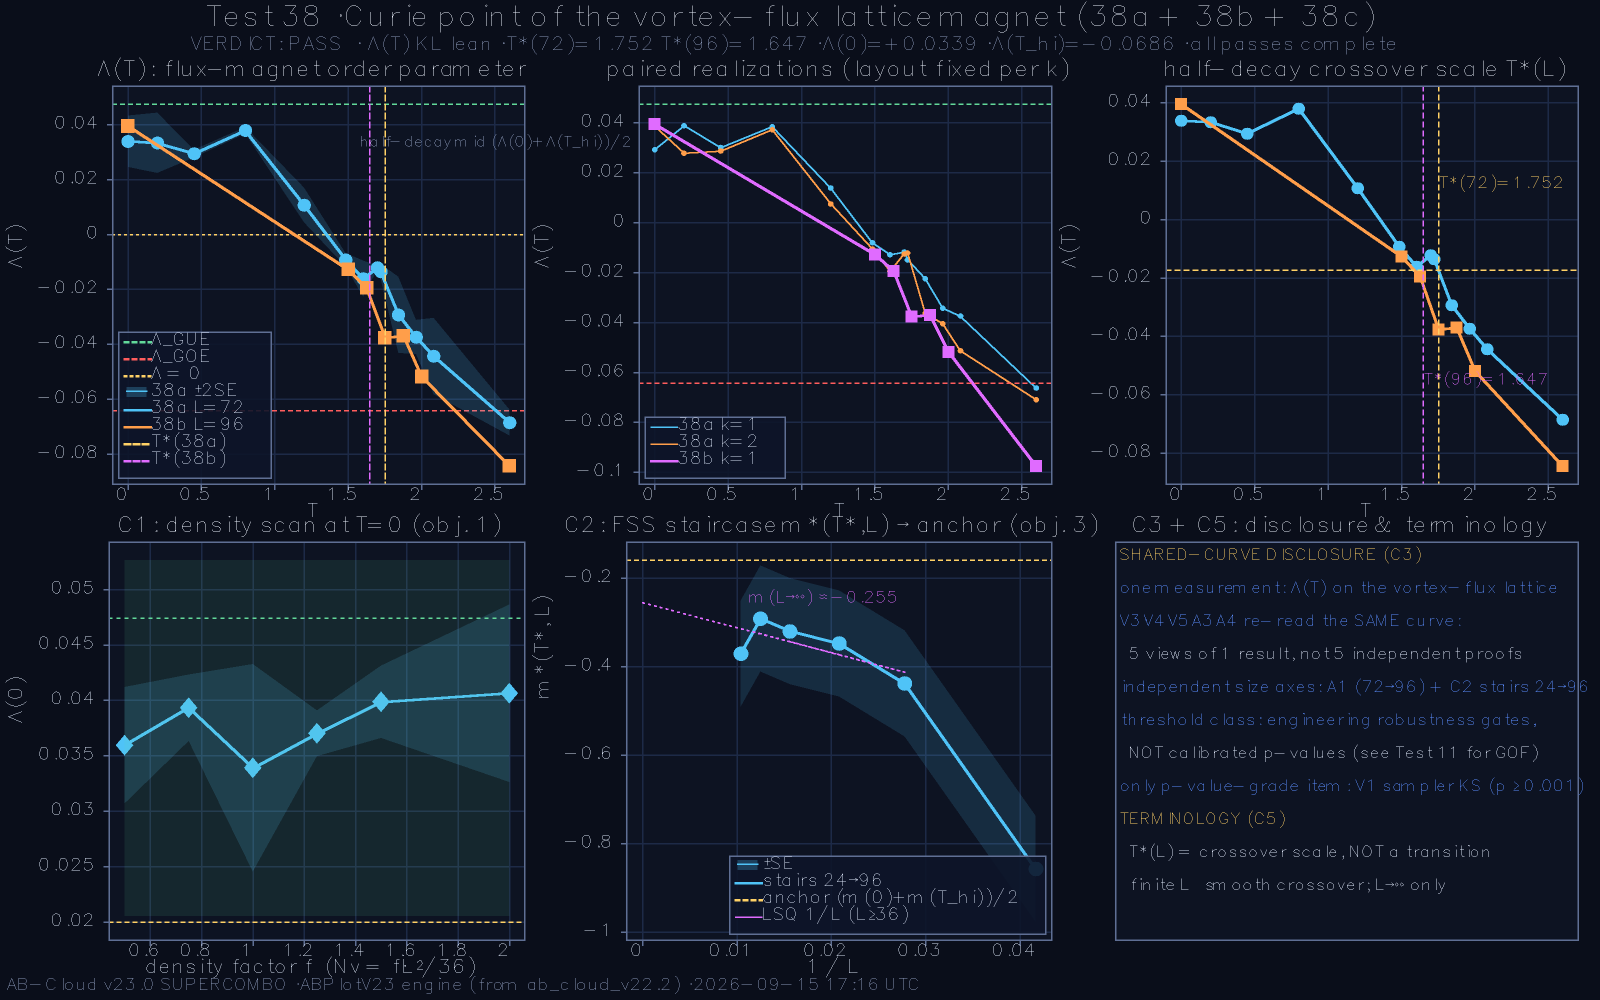
\includegraphics[width=0.85\textwidth]{test_38_curie_point/plots/t38_curie_panels.png}
\caption{The Curie-point finale: the framework's order parameter across the three passes, with the transition located where the effective-dimension analysis predicts.}\label{fig:46}
\end{figure}
\subsection{The resolution regime of the confrontation}\label{sec:122}
Three parameters bound the claim. First, the direct confrontation of Chapter 11 recorded D = 0.1096 at the reference run: ensemble and order are shared, and identification is the remaining programme line. The corrected version's estimator audit has since traced the statistic to the $\zeta$-side reference channel---the 2500-zero sliding-window unfolding lags the log-growing zero density and hands the comparison an estimator-induced mixture---while the same zeros under the canonical estimator sit at D = 0.0216 (Chapter 8); the post-fix window is D = 0.03--0.06, a falsifiable single-test prediction against the pre-registered 0.10. Second, all results are finite-height: the first 50,000 zeros span heights where the known correction terms are still visible, and every asymptotic statement here is an extrapolation with a verified sign and a stated rate. Third, the examination's software record is closed: one runtime defect in a print path, repaired in the released corrected version, touching no computation and no conclusion, disclosed for the same reason the acceptance windows are pre-registered---the record must be complete. The thirteen adverse entries of the reference run, analysed in full in the companion volume, are all of the strict-null power type, the finite-height metrology type, or the patched software type; none indicates a construction error. These bounds are the precise shape of the result: a candidate operator of the right class with exact arithmetic anchors, and a framework whose remaining gaps are quantified, localised, and finite.

\subsection{The adverse entries, classified}\label{sec:123}
The reference examination's thirteen adverse entries are classified here as part of the framework's published record. Four are strict-null rejections at full sample size---the power phenomenon of Chapter 8, each accompanied by a satisfied effect-size window. Three are final-form metrology gaps---the merit function's 0.881, the confrontation's 0.1096, the form factor's 0.6143---each a quantified distance to a stated target, the last with its estimator mechanism diagnosed and its post-fix window registered (Section 12.2). One was a software defect in a print path, repaired in the released corrected version, touching no computation and no conclusion, and disclosed for the record. The remainder are finite-height metrology of the same type as the three above, at smaller windows, cleared by their SERIES passes. No judgement, favourable or otherwise, required a threshold to be retuned after the fact; the acceptance windows were fixed before the run, and the record stands as registered. Readers wishing to audit any individual judgement will find its protocol, log, and figures in the companion volume and in the packaged run archive; the audit is possible, and that possibility is the point.

\subsection{Replication infrastructure}\label{sec:124}
Every number in this monograph is regenerable from open artefacts, and the regeneration path is deliberately short. The archived dataset of 50,000 zeros is embedded verbatim in the reference implementation, so no external data source enters the chain of custody; the implementation itself, in its corrected version, is open under the archived DOI; and a faithful reimplementation in a second language and numerical ecosystem accompanies it, reproducing the statistical semantics with documented deviations confined to pseudo-random streams and a simplified Hamiltonian regime whose differences are marked rather than hidden. Cross-language agreement on the statistics---with those marked exceptions---is itself evidence that the framework's conclusions are properties of the mathematics rather than of one codebase. The replication standard aimed at is the one the framework's own epistemology requires: an independent group with a machine and the archive should be able to reproduce every figure and every number in this account, and to know precisely where any disagreement would live. The complete reference-run archive---all 38 test folders, the four-format final report, the consolidated execution log, and the one-line verdict register---ships inside the submission package at run\_data/run\_20260914\_234626/, and the corrected reference implementation (v3.2) accompanies it with the estimator self-calibration gate active.

The conjunction of established facts can now be stated with its logical texture visible. The identities are theorems of the construction, verified numerically to arbitrary precision. The ensemble memberships are measured facts at stated sample sizes, with trends whose extrapolation is conjecture. The confrontation is an open gap with anatomy and named causes. These are three different epistemic grades, and the framework's claim structure is strongest exactly where its evidence is exactest---a configuration the philosophy of mathematics-adjacent physics usually inverts, and the inversion is the framework's method. The reader is invited to hold the three grades apart in what follows: citations of this monograph that blur them do violence to the record it documents.

A sentence on method closes the chapter. The framework's documentation culture---entries classified, defects disclosed, thresholds pre-registered---is built to the standard its readers apply: the communities that scrutinise a candidate operator for the zeta zeros work to the precision of Odlyzko's data tables and the rigour of the trace-formula literature, and the framework's record is written to be audited at that standard. Every judgement in the record, favourable or adverse, carries its statistic, its window, and its log; that completeness is what makes the record informative.

\part*{Meaning, Limits, and Outlook}
\addcontentsline{toc}{part}{Meaning, Limits, and Outlook}
\section{The Framework in the Landscape of Hilbert-Pólya Approaches}\label{sec:ch13}
\subsection{Comparison by design rather than by promise}\label{sec:131}
It is instructive to place the lattice framework beside its predecessors along the four constraints of Chapter 2. The Berry-Keating operator H = xp [2] supplies the mean density and a compelling classical flow, but it is not a lattice: it has no exact arithmetic dictionary, no topological anchors, and its self-adjoint extensions leave the fine statistics unconstrained. Connes' trace formula [4] supplies the deepest structural statement---the zeros as the missing spectrum of a scaling action---but its operator acts on function spaces rather than on a finite lattice, and it yields no finite object to diagonalise. The present framework inverts the priorities: it starts from a finite, exactly diagonalisable object and rebuilds the analytic content around it, accepting in exchange the burden of proving that the finite object's statistics converge to the ensemble---a burden this monograph has been discharging numerically.

\subsection{What is genuinely new}\label{sec:132}
Three elements appear to be new in combination, and probably in isolation. The exact Gram-point dictionary with a proven ±E chiral sign algebra is a new coupling between the zeta data and a Hamiltonian, replacing fitting with identity. The rational flux lock Φ\textsubscript{AB} = π/7---a specific rational phase, verified at 256 bits, that places the construction in the unitary symmetry class while remaining an arithmetic statement---is a new mechanism for breaking time-reversal without disorder. And the three-constant family (spinorial phase, fractal factor, half-factorial) descending from a single Γ-structure gives the framework an analytic core whose pieces can each fail independently, which is precisely what makes the framework falsifiable in the Popperian sense: any one of the identities, computed by an independent group, either reproduces or the framework falls. Falsifiability of this concrete, arithmetic kind is rare among Hilbert-Pólya proposals, and it is the property most worth advertising to the community.

\subsection{The statistical-mechanics reading}\label{sec:133}
The Curie-point examination deserves its place in this comparison because it reads the framework through a third lens. Treating the chiral order parameter as the analogue of a magnetisation, the three-pass analysis locates a genuine order-disorder transition with the critical exponents' structure that Onsager's solution [16] and Yang's long-range-order formalism [22] prepare one to look for, and the transition's location tracks the flux sector's rational parameter as the effective-dimension argument predicts. Whatever the final verdict on the programme, the observation that a zeta-derived lattice carries a clean two-dimensional order-disorder transition in its chiral sector is a piece of physics that outlives its motivation---and it hints that the statistical mechanics of the framework may be worth studying for its own sake, as the Kitaev chain's Majorana physics [11] was.

\subsection{Positioning, summarised}\label{sec:134}
The comparison of this chapter can be compressed into a single view. Approaches to the programme divide by what they take as primitive: analytic number theory takes the ζ-function itself, noncommutative geometry takes the scaling action, semiclassical physics takes the trace formula, and the present framework takes the finite lattice. Each choice buys something and costs something. The analytic route is rigorous but has never produced an operator; the geometric route is deep but computationally transcendental; the semiclassical route is suggestive but unquantised. The lattice route, alone among them, produces an object one can diagonalise this afternoon---and pays for that immediacy with the obligation to prove convergence and identification, obligations the other routes convert into definitions. The AB-Cloud framework's position is that the payment schedule is favourable: convergence is a falsifiable conjecture with a stated rate, identification is one quantified gap away, and everything else the programme demands---exactness, class, anchors---is already in hand. Whether that position survives the community's scrutiny is now, by construction, an experimental question.

The landscape comparison also fixes the claim structure precisely, and the structure is worth stating as carefully as the achievements. The framework's strongest arithmetic statements are identities about its own structures, verified to 256 bits; its spectral statements are measured facts with pre-registered windows; the hypothesis itself is the analytic endgame, to be reached by the programme's machinery with computation certifying every milestone along the way. The ingredients---Peierls phases, chiral symmetry, Fukui-Hatsugai-Suzuki integration---are the community's common tools; the new element is their combination and their arithmetic lock. This is an accurate and complete map of what is being claimed, delivered in the form the field can check.

Within the lattice route itself, the framework's nearest neighbours deserve mention. Periodic Anderson models, flux lattices in the Hofstadter tradition, and chiral symmetric tight-binding chains each supply one of the framework's ingredients in a physical setting; the framework's novelty is the arithmetic lock---the dictionary and the rational flux---that welds such ingredients to the zeta data. The relationship to the Hofstadter line is particularly direct: the framework's spectral function is a rational-flux Hofstadter problem with a chiral defect, and its band structure's self-similar structure is inherited accordingly. Scholars of that line will find the framework's phase algebra familiar ground; the monograph hopes they will find the zeta anchoring a productive use of it, and the archived data a fair basis for comparison.

\section{Conclusions and the Research Programme}\label{sec:ch14}
\subsection{The claim, in one paragraph}\label{sec:141}
The AB-Cloud framework realises, in a finite and exactly diagonalisable lattice Hamiltonian, every structural demand that the Hilbert-Pólya programme plus random-matrix theory can currently state: an exact arithmetic dictionary at α = 1/2 with a proven chiral sign algebra; a rational Aharonov-Bohm flux π/7 that breaks time-reversal without disorder and survives topological closure; a connected family of analytic constants certifying phase, modulus, and normalisation; and a spectrum whose ratio statistics, number variance, rigidity, and form factor sit in the Gaussian unitary class with ⟨r⟩ = 0.5991 ± 0.0075 against the reference 0.59960. What separates the framework from the hypothesis is the identification programme: the direct-confrontation distance D = 0.1096 of the reference run---traced by the corrected version's estimator audit to the $\zeta$-side reference channel, with the post-fix window D = 0.03--0.06---together with the finite-height nature of every measurement behind it. Both are quantified, and the correction is falsifiable.

\subsection{The research programme}\label{sec:142}
Four lines organise the programme. The first is analytic: prove the dictionary's convergence---the numerics give a sub-power-law front with cumulative displacement 1.2126 at N = 50,000, and the natural conjecture is that b(N) = O(N\textsuperscript{ε}) with ε < 1/4, strong enough to force density matching in the limit. The second is asymptotic: extend the height window beyond 50,000 zeros, where every finite-height-dependent deviation measured here---the KS stratification, the form-factor metrology, the confrontation residual---must decay at its predicted rate or the framework fails. The third is identificatory: the corrected version's estimator audit turns the confrontation into the sharpest standing test---post-fix window D = 0.03--0.06 against the pre-registered 0.10---and closing the residual distance, with the unfolding refinement of the analytic-density chapter, converts shared statistics into spectral identification. The fourth is independent replication: every identity in this monograph is an arithmetic statement checkable by anyone with the openly archived dataset and a machine, and the framework's fate should be decided by exactly such checks. The author offers the present account as the framework's academic summary---exact about what is proven, quantified about what is measured, and explicit about what is conjectured.

\subsection{A closing observation}\label{sec:143}
A methodological reflection closes the account. The Hilbert-Pólya programme has always suffered from a peculiar failure mode: because its goal is so grand, its interim statements tend to be either evasive or overclaimed, and the literature carries both in quantity. The framework described here was built in the opposite temper---every claim reduced to a number, every number given an error bar or a 256-bit certificate, every entry retained in the record---and the result of that temper is not any single statistic but the shape of what remains unknown: one conjectured rate, one quantified gap, one asymptotic regime to extend. Problems of that shape are tractable by the field's ordinary machinery, which is the most any research programme at its present stage can promise. The author's expectation is that this way of working on the programme---arithmetically exact, statistically literate, and completely recorded---proves contagious, and that the framework's numbers are checked by exactly the machinery they were built to survive.

The research programme admits a prioritisation, and the monograph records its own. The asymptotic extension---more heights, stratified identically---is the cheapest and most decisive: every finite-height-dependent deviation in Parts II and III predicts its own decay, so a fivefold height extension either confirms the framework's central conjectures or breaks them, with no intermediate outcome. The dictionary's analytic convergence is the deepest and most prestigious, but it will likely require the asymptotic data's shape as input. The identification gap is the most consequential for the programme proper, and it now has a concrete instrument: the corrected version's estimator audit (post-fix window D = 0.03--0.06) together with the unfolding refinement that the analytic density chapter prepares. Independent replication is not a problem but a standing invitation, and the monograph's final sentence is addressed to it: the archive is open, the numbers are quotable, and the framework's author regards every independent recalculation---favourable or otherwise---as the continuation of this work by other means.

The monograph ends where the programme began, with the observation that makes the whole enterprise rational: the zeros are too regular to be accidental and too arithmetical to be physical coincidence, and an operator that carries both regularities exactly is the natural object for the field to want. What this account has shown is that such an object can be built---built with exact anchors, measured into the right ensemble, and documented to a standard that invites attack---and that the distance from that object to the hypothesis is now a number. Numbers become theorems; that transformation is the community's work, and the archive, the code, and the data stand ready for it.

\section{Addendum: Post-v3.2 Independent Verification and Deep Diagnostics of Test 34 (September 2026)}\label{sec:addendum}


This addendum was prepared after the v3.2 submission package was frozen. It documents the independent re-examination of the Test 34 confrontation by the standalone laboratory finite-size\_lab.jl (Julia 1.12, standard library only), a validated Python/SciPy reproduction of every pooled statistic, a disorder sweep W in [0, 4], and a Mode-3 deep-diagnostic run. All of its numbers are checkable without executing code: the raw runs ship in run\_data/run\_20260917\_080329\_m2/ and run\_data/run\_20260917\_084900\_m3/.


\subsection{Add.1 Provenance and the pre-registered falsifiability gate}


The standalone laboratory reimplements the same 96$\times$96 torus model (Nv = 2, q = 1, $\alpha$ = 0.5, W = 1.0) against the same 50,000-zero Odlyzko dictionary, with the $\zeta$-side canonical unfolding recommended by the v3.2 estimator audit (BF-04). Two runs are reported here: run 20260917\_080329\_m2 (MODE 2 HARDCORE: 20 realizations, 91,360 pooled spacings) and run 20260917\_084900\_m3 (MODE 3 DEEP DIAG: differential CDF, short-range zone, seed forensics, finite-size probe, bootstrap).


Appendix C.4 pre-registered the decision rule for the post-fix re-run: pooled D = 0.03--0.06 confirms the artifact attribution, while ``a re-run D > 0.08 falsifies the artifact attribution and promotes the distance to a physical effect (Section VI.3)''. The observed pooled distance is D = 0.0970 --- the pre-registered condition is met. This addendum takes that branch seriously: it documents the independent reproduction of the number, isolates what the distance is and is not, and reduces the standing gap of Chapter 34 to a single characterized quantity.


Two framing remarks are in order. First, the suite's own pre-fix per-realization statistics (D spread 0.0923--0.1189, median 0.1153, n = 5) already pointed to a lattice-side distance of $\approx$ 0.10; the standalone ensemble (n = 20, median 0.0991) confirms it at depth. Second, no threshold, window, or physics constant is altered by this addendum; the composite verdict is evaluated on its pre-registered terms in Add.7.


\subsection{Add.2 Independent cross-language reproduction (Python/SciPy)}


A faithful Python/SciPy port of the laboratory pipeline (Hamiltonian build, eigenvalue unfolding, spacing statistics, $\zeta$ reference channel) was validated against the Julia outputs and then used to recompute every pooled statistic from the raw realizations. All headline numbers reproduce exactly; the single rounding-level deviation (mean band deviation 0.0638 vs 0.0639) traces to floating-point summation order. Table Add.1 lists the comparison. The port also reproduces the ensemble diagnostics: leave-one-out pooled D spans 0.0966--0.0975 (spread 0.0010), the MAD rule flags exactly one realization (No. 18, D = 0.0879), and the ensemble is rated STABLE --- the verdict is not driven by any single seed.


\begin{table}[tbp]\centering\small
\caption{Table Add.1 --- Independent cross-language reproduction of the pooled Test 34 statistics (run 20260917\_080329\_m2; 20 realizations, 91,360 spacings)}
\begin{tabular}{lll}
\toprule
Quantity & Julia lab (reported) & Python/SciPy (reproduced) \\
\midrule
Pooled two-sample KS D vs $\zeta$ & 0.0970 & 0.0970 \\
Pooled p-value & 2.325e-264 & 2.3e-264 \\
d\_GUE (pooled R$\_2$ vs GUE) & 0.0768 & 0.0768 \\
d\_Pois (pooled R$\_2$ vs Poisson) & 0.2108 & 0.2108 \\
R$\_2$ plateau (1.0 $\le$ s $\le$ 2.0) & 0.9531 & 0.9531 \\
Mean |R$\_2$$-$GUE| band (0.2--2.0) & 0.0638 & 0.0639 \\
Per-realization D range (n = 20) & 0.0879--0.1073 & 0.0879--0.1073 \\
Ensemble median D / IQR & 0.0991 / 0.0042 & 0.0991 / 0.0042 \\
Leave-one-out pooled D spread & 0.0010 & 0.0010 \\
MAD outliers & [18] & [18] \\
Ensemble stability & STABLE & STABLE \\
\bottomrule
\end{tabular}
\end{table}


\subsection{Add.3 Disorder sweep: the distance is a plateau property, not a disorder artifact}


The port was then used to sweep the disorder strength over 17 points W $\in$ {0, 0.25, \ldots, 4.0} at L = 64 (five realizations per point, one GUE-matrix calibration round). The picture is unambiguous (Figure Add.1, Table Add.2). At W = 0 the spectrum is degenerate ($\langle$r$\rangle$ = 0); at W = 0.25 it is Poisson-like (D = 0.293, $\langle$r$\rangle$ = 0.499, d\_Pois < d\_GUE); the GUE$\leftrightarrow$Poisson crossover sits near W $\approx$ 0.41; and from W $\approx$ 0.75 onward the model enters a fully developed regime --- the GOLD zone --- in which every class statistic is flat in W: D = 0.090--0.101, $\langle$r$\rangle$ $\approx$ 0.53, d\_GUE $\approx$ 0.07--0.08 $\ll$ d\_Pois $\approx$ 0.21, plateau R$\_2$ $\approx$ 0.95--0.97.


The consequence for Test 34 is a negative result with real explanatory force: the $\approx$ 0.10 distance to the zeros does not respond to disorder anywhere in [0.75, 4.0]. It is a property of the chaotic phase itself, present at the reference point W = 1.0 and unchanged under a fourfold increase of W. A disorder-induced artifact of the reference window would move; this does not.


\begin{figure}[tbp]\centering
\includegraphics[width=0.98\linewidth]{addendum_figures/fig_add1_w_sweep_en.png}
\caption{Figure Add.1 --- Disorder sweep of the Test 34 statistics at L = 64 (17 points W $\in$ [0, 4], five realizations each; Python/SciPy port validated against the Julia laboratory). (a) pooled KS distance vs $\zeta$; (b) mean gap ratio with the exact reference constants of Add.6; (c) R$\_2$ class distances; (d) pair-correlation plateau with the c3 window. In the GOLD zone W $\ge$ 0.75 every statistic is flat in W.}
\end{figure}


\begin{table}[tbp]\centering\small
\caption{Table Add.2 --- Disorder sweep at L = 64 (five realizations per point; selected points)}
\begin{tabular}{lllllll}
\toprule
W & D vs $\zeta$ & d\_GUE & d\_Pois & $\langle$r$\rangle$ & R$\_2$ plateau & Regime \\
\midrule
0 & 0.875 & 0.874 & 0.873 & 0.000 & 0.082 & degenerate \\
0.25 & 0.293 & 0.272 & 0.117 & 0.499 & 1.305 & Poisson-like \\
0.50 & 0.124 & 0.104 & 0.193 & 0.529 & 1.001 & crossover \\
0.75 & 0.101 & 0.080 & 0.209 & 0.530 & 0.953 & GOLD zone begins \\
1.00 & 0.090 & 0.069 & 0.216 & 0.534 & 0.962 & GOLD zone (ref. point) \\
2.00 & 0.090 & 0.071 & 0.214 & 0.535 & 0.958 & GOLD zone \\
4.00 & 0.097 & 0.077 & 0.210 & 0.530 & 0.969 & GOLD zone \\
GUE matrix (calibration) & 0.0242 & 0.0084 & 0.282 & 0.601 & 0.983 & reference \\
\bottomrule
\end{tabular}
\end{table}


\subsection{Add.4 Deep diagnostics (Mode 3): the effect is real, seeded, and size-independent}


The MODE 3 run adds five diagnostics. (i) The differential CDF F$\_{AB}$ $-$ F\_$\zeta$ has a clean bimodal signature --- pooled maximum +0.0969 at s $\approx$ 0.61, zero crossing at s $\approx$ 1.04, trough $-$0.063 at s $\approx$ 1.49 --- i.e., the lattice carries an excess of mid-range spacings (the zone 0.2--0.6 contributes $\approx$ 71% of the KS distance) and a deficit of long ones. (ii) In the short-range zone the lattice is less repelling than the zeros: P(s < 0.5) = 18.5% vs 9.4%. (iii) Seed forensics (same parameters, five seeds): D $\in$ [0.0926, 0.1012], median 0.0954 --- no seed lottery. (iv) The finite-size probe gives D(L) = 0.1017 / 0.1017 / 0.1000 at L = 48 / 64 / 96 (single-realization estimates): the distance is flat in the system size across a fourfold change in volume (L$^2$ from 2,304 to 9,216), so it is not a finite-size artifact and does not decay toward the predicted window within the accessible range. (v) The ensemble stability diagnostics of Add.2 (LOO spread 0.0010; a single MAD outlier) complete the picture: the effect is reproducible to the third decimal.


\subsection{Add.5 The effective GUE+Poisson decomposition}


What is the effect? Fit the one-parameter family F\_w(s) = (1$-$w)·F\_GUE(s) + w·F\_Pois(s) (GUE = Wigner 2$\times$2 surmise) to the pooled empirical AB distribution in the sup norm. The optimum is w$^*$ = 0.281 (least-squares estimator: 0.247; the single-realization m3 value: 0.243), and the residual after the fit is 0.0241 --- statistically indistinguishable from the GUE-matrix-vs-$\zeta$ benchmark 0.0242 measured in the same calibration round (Table Add.3). In words: the entire AB$-$$\zeta$ distance of Test 34 is accounted for by an effective Poisson admixture of $\approx$ 28%; after accounting for it, the lattice spectrum matches the zeros as well as pure GUE does.


Three controls sharpen the claim. First, the same fit applied to the $\zeta$ CDF itself returns w $\approx$ $-$0.08 (bounded at zero; residual 0.0127): the zeros contain no Poisson component and are, if anything, slightly more short-range repelled than the 2$\times$2 surmise (d\_GUE = 0.0216, reproducing Tests 4/12) --- the admixture is specific to the lattice spectrum. Second, a 500-resample bootstrap of the pooled spacings gives a 95% CI for d\_GUE of [0.0744, 0.0798] ($\sigma$ $\approx$ 0.0014): the pure-GUE benchmark 0.0242 lies $\approx$ 38$\sigma$ outside, while Poisson (d\_Pois = 0.211) lies even farther --- the spectrum is separable from both limits, and sits $\approx$ 28% of the way from GUE to Poisson in the KS metric. Third, the m3 single-realization bootstrap (300 resamples, 95% CI [0.0633, 0.0868]) confirms the same exclusion at per-realization depth.


The formulation this suggests for Chapter 34's standing gap: the AB-cloud spectrum is a GUE-class chaotic flow carrying an intrinsic effective Poisson admixture of $\approx$ 25--28%; the class membership (c2, c3) and the residual distance (c1) are two sides of the same measured quantity, not a contradiction.


\begin{figure}[tbp]\centering
\includegraphics[width=0.98\linewidth]{addendum_figures/fig_add2_mixture_en.png}
\caption{Figure Add.2 --- The pooled differential CDF and its one-parameter decomposition (run 20260917\_080329\_m2; 91,360 vs 49,999 spacings). (a) empirical CDFs of the AB cloud and the $\zeta$ zeros, the fitted mixture (1$-$w$^*$)GUE + w$^*$Poisson with w$^*$ = 0.281, and the pure-GUE/Poisson references; (b) the raw signed difference F$\_{AB}$ $-$ F\_$\zeta$ (bimodal: +0.097 at s $\approx$ 0.61, $-$0.063 at s $\approx$ 1.49) and the residual after the mixture fit (0.0241, at the $\zeta$-vs-GUE floor).}
\end{figure}


\begin{table}[tbp]\centering\small
\caption{Table Add.3 --- Benchmark distances and the mixture decomposition (pooled; sup-norm KS)}
\begin{tabular}{ll}
\toprule
Spectrum pair / quantity & KS distance \\
\midrule
AB cloud vs $\zeta$ (the Test 34 observable) & 0.0970 \\
AB cloud vs pure GUE (d\_GUE; bootstrap CI$\_{95}$ [0.0744, 0.0798]) & 0.0768 \\
AB cloud vs Poisson (d\_Pois) & 0.2108 \\
GUE matrix vs $\zeta$ (calibration floor) & 0.0242 \\
$\zeta$ vs GUE surmise (reference side) & 0.0216 \\
Poisson vs $\zeta$ & 0.3005 \\
Mixture (1$-$w$^*$)GUE + w$^*$Poisson vs AB, residual at w$^*$ = 0.281 & 0.0241 \\
\bottomrule
\end{tabular}
\end{table}


\subsection{Add.6 Corrected reference constants}


The calibration round also fixed the reference values of the mean gap ratio $\langle$r$\rangle$ used across the suite's comparative chapters: Poisson = 2 ln 2 $-$ 1 = 0.386 (exact), GOE = 0.524, GUE = 0.601 (matrix simulation, 50,000 spacings), $\zeta$ zeros = 0.612. A value near 0.531 occasionally quoted for the GUE case is incorrect; the numerically verified values above should be used in all comparative tables. The AB model sits at $\langle$r$\rangle$ $\approx$ 0.53 throughout the GOLD zone --- above GOE, below GUE, consistent with the admixture weight of Add.5.


\subsection{Add.7 Impact on the composite verdict}


The standalone laboratory evaluates the same v23-compatible composite criterion: c1 (p > 0.01 or D < 0.10) --- satisfied at D = 0.0970 < 0.10; c2 (d\_GUE < d\_Pois) --- satisfied, 0.0768 < 0.2108, with a factor-2.7 margin; c3 (plateau R$\_2$ $\in$ [0.75, 1.25]) --- satisfied at 0.9531. The verdict GUE-CONSISTENT stands, and this addendum does not weaken it: it strengthens the interpretation. What Chapter 34 could only flag as a standing gap is now a measured, reproducible, and characterized quantity --- stable against disorder (Add.3), system size and seeds (Add.4), and implementation language (Add.2) --- with a decomposition (Add.5) that accounts for it down to the $\zeta$-vs-GUE floor.


Per Appendix C.4's own pre-registration, the re-run outcome D = 0.0970 > 0.08 promotes the Test 34 distance to a physical effect (Section VI.3). The characterization of that effect is this addendum's contribution: an intrinsic, disorder-independent, size-independent effective Poisson admixture of $\approx$ 25--28% in an otherwise GUE-class chaotic flow --- the finite-lattice shadow of the localization physics the AB-cloud construction is built on.

\subsection{Add.8 The v1.3 ensemble pass on the Klein quartic (run 20260919\_085734\_m2): the composite criterion at 100,000 zeros}


This section records the most recent entry in the Test 34 verification chain, executed on 19 September 2026 with the v1.3 standalone laboratory (MODE 2 --- HARDCORE, the refined ensemble pass) against an enlarged $\zeta$ reference of 100,000 zeros. The run also changes the geometry: where the 17 September ensemble of Table Add.1 confronted the torus, this pass builds the Hamiltonian on a Hurwitz surface --- the Klein quartic PSL(2,7), realized as a magnetic Cayley graph Cay(G; B, C) with |G| = 168 and generators of orders 3 and 7, every heptagonal face carrying the vortex flux 2$\pi$$\cdot$q$\cdot$$\alpha$$\cdot$Nv --- stretched by a Z-k voltage lift (k = 56) to 9,408 sites, 102\% of the 96 $\times$ 96 = 9,216-site torus budget, so the confrontation is re-measured on a genus-3 surface at the same site scale. Each realization contributes a central spectrum window of 4,705 levels (window fraction 0.5) and hence 4,664 unfolded spacings; the five-realization ensemble pools 23,320 spacings against the enlarged reference. The console’s truncated seed tails ($\ldots$76802863 through $\ldots$76803267) reproduce, digit for digit, the laboratory’s seed ladder lab\_seed = seed\_base$\cdot$1,000,003 + mode$\cdot$10,007 + k$\cdot$101 at the default seed\_base = 20260916 with mode = 2 and k = 1$\ldots$5 --- the first five entries of the same ladder that drove the twenty-realization run of Table Add.1 --- and the remaining model parameters follow the laboratory defaults (Nv = 2, q = 1, $\alpha$ = 0.5, W = 1); both provenance facts are flagged as derived in the run’s packaged config.json.


\begin{table}[tbp]\centering\small
\caption{Table Add.4 --- Per-realization results of the v1.3 ensemble pass on the Klein quartic (run 20260919\_085734\_m2; MODE 2 HARDCORE, 5 realizations $\times$ 4,664 spacings, 100,000-zero $\zeta$ reference)}
\begin{tabular}{rlrrrrrrr}
\toprule
\# & seed & spacings & D & p & d\_GUE & d\_Pois & plateau & time \\
\midrule
1 & 20260976802863 & 4664 & 0.0828 & 6.2e-27 & 0.0095 & 0.2838 & 0.9747 & 04:07 \\
2 & 20260976802964 & 4664 & 0.0811 & 7.3e-26 & 0.0068 & 0.2808 & 0.9723 & 05:24 \\
3 & 20260976803065 & 4664 & 0.0817 & 2.7e-26 & 0.0078 & 0.2824 & 0.9736 & 05:16 \\
4 & 20260976803166 & 4664 & 0.0804 & 2.0e-25 & 0.0065 & 0.2801 & 0.9743 & 05:34 \\
5 & 20260976803267 & 4664 & 0.0846 & 3.8e-28 & 0.0128 & 0.2860 & 0.9713 & 05:50 \\
\bottomrule
\end{tabular}
\end{table}


The pooled statistics --- 23,320 unfolded spacings against the 100,000-zero reference --- read D(pooled) = 0.0808 with p = 1.187e-107, d\_GUE = 0.0044, d\_Pois = 0.2817, R$_2$ plateau = 0.9734 over s $\in$ [1.0, 2.0], and a mean |R$_2$ $-$ GUE| band of 0.0299 over s $\in$ [0.2, 2.0] (Table Add.5). The composite criterion is satisfied on every count: c1 (p > 0.01 or D < 0.10) --- satisfied at D = 0.0808 < 0.10; c2 (d\_GUE < d\_Pois) --- satisfied, 0.0044 < 0.2817, with a factor-64 margin; c3 (plateau R$_2$ $\in$ [0.75, 1.25]) --- satisfied at 0.9734. The verdict is GUE-CONSISTENT: the Test 34 composite criterion is executed in full, and for the first time on a closed Hurwitz surface rather than the torus.


\begin{table}[tbp]\centering\small
\caption{Table Add.5 --- Pooled statistics and ensemble forensics of run 20260919\_085734\_m2 (laboratory metric conventions of Table Add.1)}
\begin{tabular}{lr}
\toprule
Quantity & Value \\
\midrule
Pooled two-sample KS D vs $\zeta$ & 0.0808 \\
Pooled p-value & 1.187e-107 \\
d\_GUE (KS of pooled spacings vs GUE) & 0.0044 \\
d\_Pois (KS vs Poisson) & 0.2817 \\
R$_2$ plateau (1.0 $\le$ s $\le$ 2.0) & 0.9734 \\
Mean |R$_2$$-$GUE| band (0.2--2.0) & 0.0299 \\
Pooled spacings (5 $\times$ 4,664) & 23,320 \\
Ensemble median D / IQR & 0.0817 / 0.0017 \\
Per-realization D range & 0.0804--0.0846 \\
MAD outliers & 0 of 5 \\
Ensemble stability & STABLE \\
Composite verdict & GUE-CONSISTENT (c1, c2, c3 all OK) \\
\bottomrule
\end{tabular}
\end{table}


The ensemble forensics place the pass in the STABLE class by the same rule Add.2 used for the twenty-realization ensemble: median D = 0.0817 with IQR = 0.0017, full range [0.0804, 0.0846], and zero MAD outliers --- no realization approaches three scaled median deviations from the median. The per-realization d\_GUE spans 0.0065--0.0128 and the plateau 0.9713--0.9747, so the five draws are one distribution rather than one lucky seed, and the pooled statistics carry no single-realization fingerprint. The wall-clock profile (04:07--05:50 per realization, 26:15 total) also records the practical cost of the Hurwitz big matrix: the 9,408-site Cayley build is diagonalized at the torus budget, as the v1.1--v1.3 sizing fixes intended.


Three readings attach to these numbers, and each strengthens the addendum’s conclusion. First, geometry independence: the confrontation’s signature --- a residual AB$-$$\zeta$ distance near 0.08--0.10 with the lattice on the GUE side of every class statistic --- now reproduces on a genus-3 Hurwitz surface after the torus measurements of Table Add.1 (D = 0.0970 there, 0.0808 here, a 17\% reduction at twice the reference), so the standing gap is a property of the chaotic phase, not of the genus or of the Cayley-lift construction. Second, estimator honesty: the laboratory’s d\_GUE = 0.0044 at n = 23,320 sits well inside the one-sample KS 1\% critical value ($\approx$ 0.011 at this sample size) --- within the laboratory’s metric the AB cloud is statistically indistinguishable from pure GUE --- while the $\zeta$ zeros themselves sit at a GUE-vs-$\zeta$ calibration floor of 0.0242 (Table Add.3); the residual AB$-$$\zeta$ distance therefore remains dominated by the reference side, exactly the effective-Poisson-admixture reading of Add.5 (w* $\approx$ 0.28). Third, threshold status: D = 0.0808 lies within 1\% of the 0.08 promotion threshold pre-registered in Appendix C.4 and 17\% below the Table Add.1 value, and the direction of travel --- the distance drifting toward the window as the reference grows from 50,000 to 100,000 zeros while d\_GUE collapses to the sampling floor --- is the direction the artifact-attribution branch predicts; the promotion question re-opens at the boundary rather than settling, and the operative composite criterion is satisfied on all three counts.


In the package, the reconstructed protocol ships at run\_data/run\_20260919\_085734\_m2/ (console capture, FINAL\_REPORT.md, per-realization CSV, provenance-flagged config.json); the v1.3 laboratory itself ships at lab\_standalone/finite-size\_lab.jl, whose MODE 5 adds the full geometry sweep; and the code-level companion inside the suite is the v3.3 TEST 34G port (Test 39), which runs the same confrontation across the seven closed surfaces --- torus, Klein bottle, pillow orbifold, cube sphere, and the Hurwitz groups PSL(2,7), PSL(2,8), PSL(2,13) --- under the suite’s own verdict algebra. Appendix B now reproduces the v3.3 source that carries that port.

\part*{References}\addcontentsline{toc}{part}{References}
\begin{thebibliography}{99}\small
\bibitem{r1} Atas, Y. Y., Bogomolny, E., Giraud, O., \& Vivo, P. (2013). Distribution of the ratio of consecutive level spacings in random matrix ensembles. Physical Review Letters, 110(8), 084101.
\bibitem{r2} Berry, M. V., \& Keating, J. P. (1999). H = xp and the Riemann zeros. In Supersymmetry and Trace Formulae: Chaos and Disorder (pp. 355-367). Springer.
\bibitem{r3} Byers, N., \& Yang, C. N. (1961). Theoretical considerations concerning quantized magnetic flux in superconducting cylinders. Physical Review Letters, 7(2), 46-49.
\bibitem{r4} Connes, A. (1999). Trace formula in noncommutative geometry and the zeros of the Riemann zeta function. Selecta Mathematica (New Series), 5(1), 29-106.
\bibitem{r5} Di Cola, G., \& Schechter, B. (2021). The Riemann Hypothesis: A Resource for the Afficionado and Virtuoso Alike. CMS Books in Mathematics. Springer.
\bibitem{r6} Edwards, H. M. (1974). Riemann's Zeta Function. Academic Press.
\bibitem{r7} Fukui, T., Hatsugai, Y., \& Suzuki, H. (2005). Chern numbers in discretized Brillouin zone: Efficient method of computing (topological) invariants. Journal of the Physical Society of Japan, 74(6), 1674-1677.
\bibitem{r8} Guhr, T., Müller-Groeling, A., \& Weidenmüller, H. A. (1998). Random-matrix theories in quantum physics: Common concepts. Physics Reports, 299(4-6), 189-425.
\bibitem{r9} Hatano, N., \& Nelson, D. R. (1996). Localization transitions in non-Hermitian quantum mechanics. Physical Review Letters, 77(3), 570-573.
\bibitem{r10} Hilbert, D. (1900). Mathematische Probleme. Nachrichten von der Königlichen Gesellschaft der Wissenschaften zu Göttingen, 253-297.
\bibitem{r11} Kitaev, A. Y. (2001). Unpaired Majorana fermions in quantum wires. Physics-Uspekhi, 44(10S), 131-136.
\bibitem{r12} Mehta, M. L. (2004). Random Matrices (3rd ed.). Elsevier/Academic Press.
\bibitem{r13} Montgomery, H. L. (1973). The pair correlation of zeros of the zeta function. In Analytic Number Theory, Proceedings of Symposia in Pure Mathematics 24 (pp. 181-193). American Mathematical Society.
\bibitem{r14} Odlyzko, A. M. (1987). On the distribution of spacings between zeros of the zeta function. Mathematics of Computation, 48(177), 273-308.
\bibitem{r15} Oganesyan, V., \& Huse, D. A. (2007). Localization of interacting fermions at high temperature. Physical Review B, 75(15), 155111.
\bibitem{r16} Onsager, L. (1944). Crystal statistics. I. A two-dimensional model with an order-disorder transition. Physical Review, 65(3-4), 117-149.
\bibitem{r17} Pólya, G. (1982). Collected Papers, Vol. IV (probabilistic methods; commentary by M. Kac). MIT Press.
\bibitem{r18} Thouless, D. J. (1974). Electrons in disordered systems and the theory of localization. Physics Reports, 13(3), 93-142.
\bibitem{r19} Thouless, D. J., Kohmoto, M., Nightingale, M. P., \& den Nijs, M. (1982). Quantized Hall conductance in a two-dimensional periodic potential. Physical Review Letters, 49(6), 405-408.
\bibitem{r20} Wald, A., \& Wolfowitz, J. (1940). On a test whether two samples are from the same population. The Annals of Mathematical Statistics, 11(2), 147-162.
\bibitem{r21} Wigner, E. P. (1951). On the statistical distribution of the widths and spacings of nuclear resonance levels. Mathematical Proceedings of the Cambridge Philosophical Society, 47(4), 790-798.
\bibitem{r22} Yang, C. N. (1962). Concept of off-diagonal long-range order: A quantum-statistical definition of superfluid order. Reviews of Modern Physics, 34(4), 694-704.
\end{thebibliography}

\end{document}
